\chapter{Additional Material for Chapter 5}
\graphicspath{{figures/ch_5/}}
\addtocontents{toc}{\protect\setcounter{tocdepth}{0}}

\section{Simulation Model}
\label{ch_5:sec:full_simulation_model_explanation}

Data for the simulation study in Section~\ref{ch_5:subsec:simulation} are generated from a two strain model, which is described in the main text.
Here, we present the mathematical details of the model presented in Figure~\ref{ch_5:fig:full_model_diagram_compact}.
We first present the rates of transitions between compartments in the model in \eqref{ch_5:eqn:transition_rates_simulation_model}, where the interpretation and values of the parameters used in the simulation are given in Table~\ref{ch_5:tbl:simulation_parameters_and_interpretations}.
Using the transition rates in \eqref{ch_5:eqn:transition_rates_simulation_model}, we define the ODEs in the model in \eqref{ch_5:eqn:ODEs_simulation_model}, subject to the initial conditions given in Table~\ref{ch_5:tbl:simulation_parameters_and_interpretations}.

We use the solutions to the system of differential equations to simulate the six time series referenced in Section~\ref{ch_5:subsec:surveillance}  according to \eqref{ch_5:eqn:case_emission_simulation}--\eqref{ch_5:eqn:new_variant_emission_simulation}.
The time series of counts of new sequences from the old variant \( \left( \bV^O \right) \) and the novel variant \( \left( \bV^N \right) \) are summed to create the time series of counts of all variants \( \left( \bV^A \right) \).

The simulated data for the medium takeover speed scenario is plotted in Figure~\ref{ch_5:fig:simulated_binned_data_medium_plot}, with the gray shaded areas indicating the time points for which we produce forecasts.
Similar figures for the other data sets are presented in Figures~\ref{ch_5:fig:simulated_binned_data_slow_plot} and \ref{ch_5:fig:simulated_binned_data_fast_plot}.

\begin{equation}
\begin{aligned}
\lambda_{S_A E_O}(S_A, I_O)  =&  \frac{\beta_O}{N} S_A I_O,   \\
\lambda_{S_A E_N}(S_A, I_N)  =&  \frac{\beta_N}{N} S_A I_N,   \\
\lambda_{E_O I_O}(E_0)  =& \gamma E_O,    \\
\lambda_{I_O H_O}(I_O)  =& \nu \tau I_O,   \\
\lambda_{I_O R_O}(I_O)  =& \nu \left( 1 - \tau \right) I_O,   \\
\lambda_{H_O U_O}(H_O)  =& \eta  \upsilon H_O,   \\
\lambda_{H_O R_O}(H_O)  =& \eta  \left( 1 - \upsilon \right) H_O,   \\
\lambda_{U_O D_A}(U_O)  =& \omega \chi U_O, \\
\lambda_{U_O R_O}(U_O)  =& \omega \left( 1 - \chi \right) U_O, \\
\lambda_{R_O S_A}(R_O)  =& \kappa R_O, \\
\end{aligned}
\qquad \quad \quad
\begin{aligned}
\lambda_{R_O E_N}(R_O, I_N)  =& \epsilon \frac{\beta_N}{N} R_O I_N, \\
\lambda_{S_N E_N}(S_N, I_N)  =&  \frac{\beta}{N} S_N I_N,   \\
\lambda_{E_N I_N}(E_N)  =& \gamma E_N,    \\
\lambda_{I_N H_N}(I_N)  =& \nu \tau I_N,   \\
\lambda_{I_N R_N}(I_N)  =& \nu \left( 1 - \tau \right) I_N,   \\
\lambda_{H_N U_N}(H_N)  =& \eta  \upsilon H_N,   \\
\lambda_{H_N R_N}(H_N)  =& \eta  \left( 1 - \upsilon \right) H_N,   \\
\lambda_{U_N D_A}(U_N)  =& \omega \chi U_N, \\
\lambda_{U_N R_N}(U_N)  =& \omega \left( 1 - \chi \right) U_N, \\
\lambda_{R_N S_N}(R_N)  =& \kappa R_N, \\
\end{aligned}
\label{ch_5:eqn:transition_rates_simulation_model}
\end{equation}

\begin{xltabular}{\columnwidth}{c>{\RaggedRight}Xr}
\label{ch_5:tbl:simulation_parameters_and_interpretations}\\
\caption{TKTK}\\[\belowcaptionskip]
\thead{Parameter} & \thead{Interpretation} & \thead{Value} \\ \hline
\( \beta_{O} \)  & Contact rate for old variant & 1.5 \\
\( \beta_{N} \)  & Contact rate for novel variant &  see Table~\ref{ch_5:table:scenario_differing_parameters} \\
\( \epsilon \) & Parital immunity to novel variant conferred by old variant & see Table~\ref{ch_5:table:scenario_differing_parameters} \\
\( 1 / \nu \) & Mean infectious period duration (weeks) & 5 / 7 \\
\( 1 / \gamma \) & Mean latent period duration (weeks) & 2 / 7 \\
\( 1 / \eta \) & Mean hospitalization duration (weeks) & 3 / 7 \\
\( 1 / \omega \) & Mean ICU stay duration (weeks) & 5 / 7 \\
\( 1 / \kappa \) & Mean immunity duration (weeks) & 20 \\
\( \tau \) & Infection-hospitalization ratio & 0.02 \\
\( \upsilon \) & Hospitalization-ICU admission ratio & 0.15 \\
\( \chi \) & ICU-fatality ratio & 0.15 \\
\( \rho^W \) & Case detection rate & 0.2 \\
\( \rho^Z \) & Death detection rate & 0.9 \\
\( \rho^V \) & Sequence detection rate (relative to cases) & 0.1 \\
\( \phi_W \) & Over-dispersion for observed new cases & 100 \\
\( \phi_X \) & Over-dispersion for observed hospitalizations & 100 \\
\( \phi_Y \) & Over-dispersion for observed ICU & 100 \\
\( \phi_Z \) & Over-dispersion for observed new deaths & 100 \\
\( \phi_V \) & Over-dispersion for observed new sequences & 100 \\
\( S_{A,0} \) & Initial size of population susceptible to all variants & 1,899,600 \\
\( E_{O,0} \) & Initial size of population infected, but not yet infectious with the old variant & 100 \\
\( I_{O,0} \) & Initial size of population infectious with the old variant & 300 \\
\( R_{O,0} \) & Initial size of population recovered from the old variant & 300 \\
\( S_{N,0} \) & Initial size of population susceptible to only the novel variant & 0 \\
\( E_{N,0} \) & Initial size of population infected, but not yet infectious with the novel variant & 0 \\
\( I_{N,0} \) & Initial size of population infectious with the novel variant & 0 \\
\( R_{N,0} \) & Initial size of population recovered from the novel variant & 0 \\
\( H_{O,0} \) & Initial size of population hospitalized with the old variant & 0 \\
\( H_{N,0} \) & Initial size of population hospitalized with the novel variant & 0 \\
\( U_{O,0} \) & Initial size of population in the ICU with the old variant & 0 \\
\( U_{N,0} \) & Initial size of population in the ICU with the novel variant & 0 \\
\( D_{A,0} \) & Initial size of population deceased due to infection from all variants & 0
\end{xltabular}

\begin{equation}
\begin{aligned}
\deriv{S_A}{t}    =&  \lambda_{R_O S_A}(R_O) - \left( \lambda_{S_A E_O}(S_A, I_O) + \lambda_{S_A E_N}(S_A, I_N) \right), \\
\deriv{E_O}{t}    =&  \lambda_{S_A E_O}(S_A, I_O) - \lambda_{E_O I_O}(E_0),    \\
\deriv{I_O}{t}    =&  \lambda_{E_O I_O}(E_0) - \left( \lambda_{I_O H_O}(I_O)  + \lambda_{I_O R_O}(I_O) \right),\\
\deriv{H_O}{t}    =&  \lambda_{I_O H_O}(I_O) - \left( \lambda_{H_O U_O}(H_O)  +  \lambda_{H_O R_O}(H_O) \right),\\
\deriv{U_O}{t}    =&  \lambda_{H_O U_O}(H_O) - \left( \lambda_{U_O D_A}(U_O)  + \lambda_{U_O R_O}(U_O) \right),\\
\deriv{R_O}{t}    =&  \lambda_{I_O R_O}(I_O) + \lambda_{H_O R_O}(H_O) + \lambda_{U_O R_O}(U_O) - \left( \lambda_{R_O S_A}(R_O) + \lambda_{R_O E_N}(R_O, I_N) \right),    \\
\deriv{S_N}{t}    =&  \lambda_{R_N S_N}(R_N) - \lambda_{S_N E_N}(S_N, I_N), \\
\deriv{E_N}{t}    =&  \lambda_{S_N E_N}(S_N, I_N) + \lambda_{R_O E_N}(R_O, I_N) + \lambda_{S_N E_N}(S_N, I_N) - \lambda_{E_N I_N}(E_N)\,    \\
\deriv{I_N}{t}    =&  \lambda_{E_N I_N}(E_0) - \left( \lambda_{I_N H_N}(I_N)  + \lambda_{I_N R_N}(I_N) \right),\\
\deriv{H_N}{t}    =&  \lambda_{I_N H_N}(I_N) - \left( \lambda_{H_N U_N}(H_N)  +  \lambda_{H_N R_N}(H_N) \right),\\
\deriv{U_N}{t}    =&  \lambda_{H_N U_N}(H_N) - \left( \lambda_{U_N D_A}(U_N)  + \lambda_{U_N R_N}(U_N) \right),\\
\deriv{R_N}{t}    =&  \lambda_{I_N R_N}(I_N) + \lambda_{H_N R_N}(H_N) + \lambda_{U_N R_N}(U_N) - \lambda_{R_N S_N}(R_N),    \\
\deriv{D_A}{t}    =&  \lambda_{U_O D_A}(U_O) + \lambda_{U_N D_A}(U_N) \\
\label{ch_5:eqn:ODEs_simulation_model}
\end{aligned}
\end{equation}

\begin{equation}
\begin{aligned}
W_l \sim \operatorname{Negative Binomial} & \left( \mu^{W}_l = \rho^W \cdot N \cdot \left( \Delta N_{E_O I_O} \left( t_l \right) + \Delta N_{E_N I_N} \left( t_l \right) \right) \right.,\\
& \left. \left(\sigma^W_l\right)^{2} = \mu^{W}_l \left( 1 + \mu^{W}_l / \phi_W \right) \right)
\end{aligned}
\label{ch_5:eqn:case_emission_simulation}
\end{equation}
\begin{equation}
X_l \sim \operatorname{Negative Binomial} \left( \mu^{X}_l = N \cdot \left( H_O \left( t_l \right) + H_N \left( t_l \right) \right), \left(\sigma^X_l\right)^{2} = \mu^{X}_l \left( 1 + \mu^{X}_l / \phi_X \right) \right)
\label{ch_5:eqn:hosp_emission_simulation}
\end{equation}
\begin{equation}
Y_l \sim \operatorname{Negative Binomial} \left( \mu^{Y}_l = N \cdot \left( U_O \left( t_l \right) + U_N \left( t_l \right) \right), \left(\sigma^Y_l\right)^{2} = \mu^{Y}_l \left( 1 + \mu^{Y}_l / \phi_Y \right) \right)
\label{ch_5:eqn:icu_emission_simulation}
\end{equation}
\begin{equation}
\begin{aligned}
Z_l \sim \operatorname{Negative Binomial} & \left( \mu^{Z}_l = \rho^Z \cdot N \cdot \left(\Delta N_{U_O D_O} \left( t_l \right) + \Delta N_{U_N D_N} \left( t_l \right) \right),\right. \\
& \left. \left(\sigma^Z_l\right)^{2} = \mu^{Z}_l \left( 1 + \mu^{Z}_l / \phi_Z \right) \right)
\label{ch_5:eqn:death_emission_simulation}
\end{aligned}
\end{equation}
\begin{equation}
    V^O_l \sim \operatorname{Negative Binomial} \left( \mu^{V^O}_l = \mu^{W}_l \cdot \left( 1 - \delta\left(t_l\right)\right) \cdot \rho^V , \left(\sigma^Z_l\right)^{2} = \mu^{V^O}_l \left( 1 + \mu^{V^O}_l / \phi_V \right) \right)
\label{ch_5:eqn:old_variant_emission_simulation}
\end{equation}
\begin{equation}
    V^N_l \sim \operatorname{Negative Binomial} \left( \mu^{V^N}_l = \mu^{W}_l \cdot \delta\left(t_l\right) \cdot \rho^V , \left(\sigma^Z_l\right)^{2} = \mu^{V^O}_l \left( 1 + \mu^{V^N}_l / \phi_V \right) \right)
\label{ch_5:eqn:new_variant_emission_simulation}
\end{equation}

\begin{figure}
    \centering
    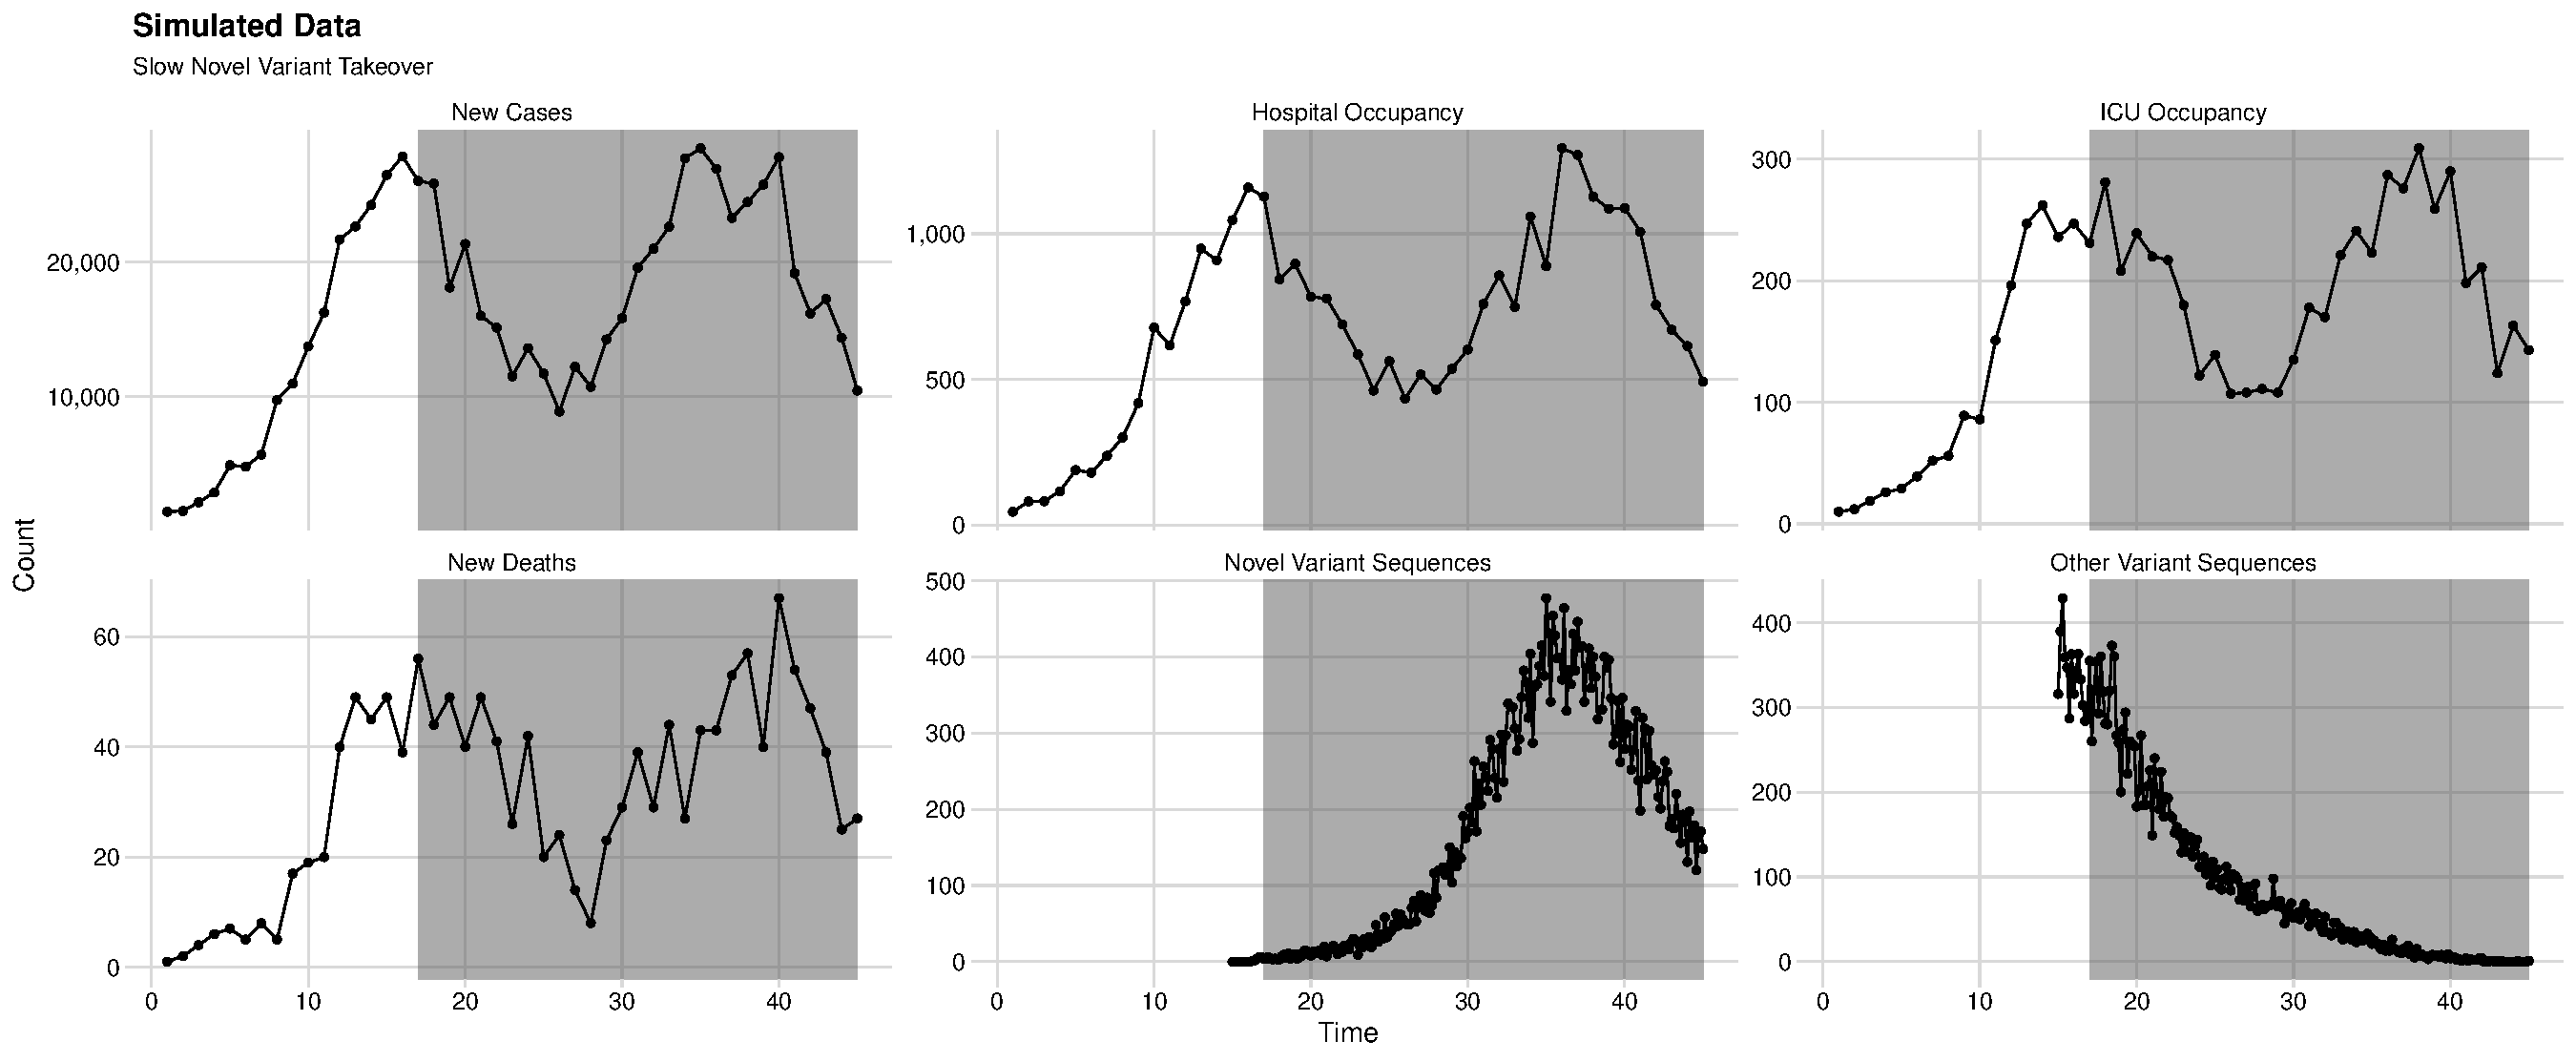
\includegraphics[width=1.0\columnwidth]{simulated_binned_data_slow_plot}
    \caption[Simulated data set for the slow takeover speed scenario.]{Simulated data set for the slow takeover speed scenario.
    The gray shaded areas indicate the time points for which we create forecasts}
    \label{ch_5:fig:simulated_binned_data_slow_plot}
\end{figure}

\begin{figure}
    \centering
    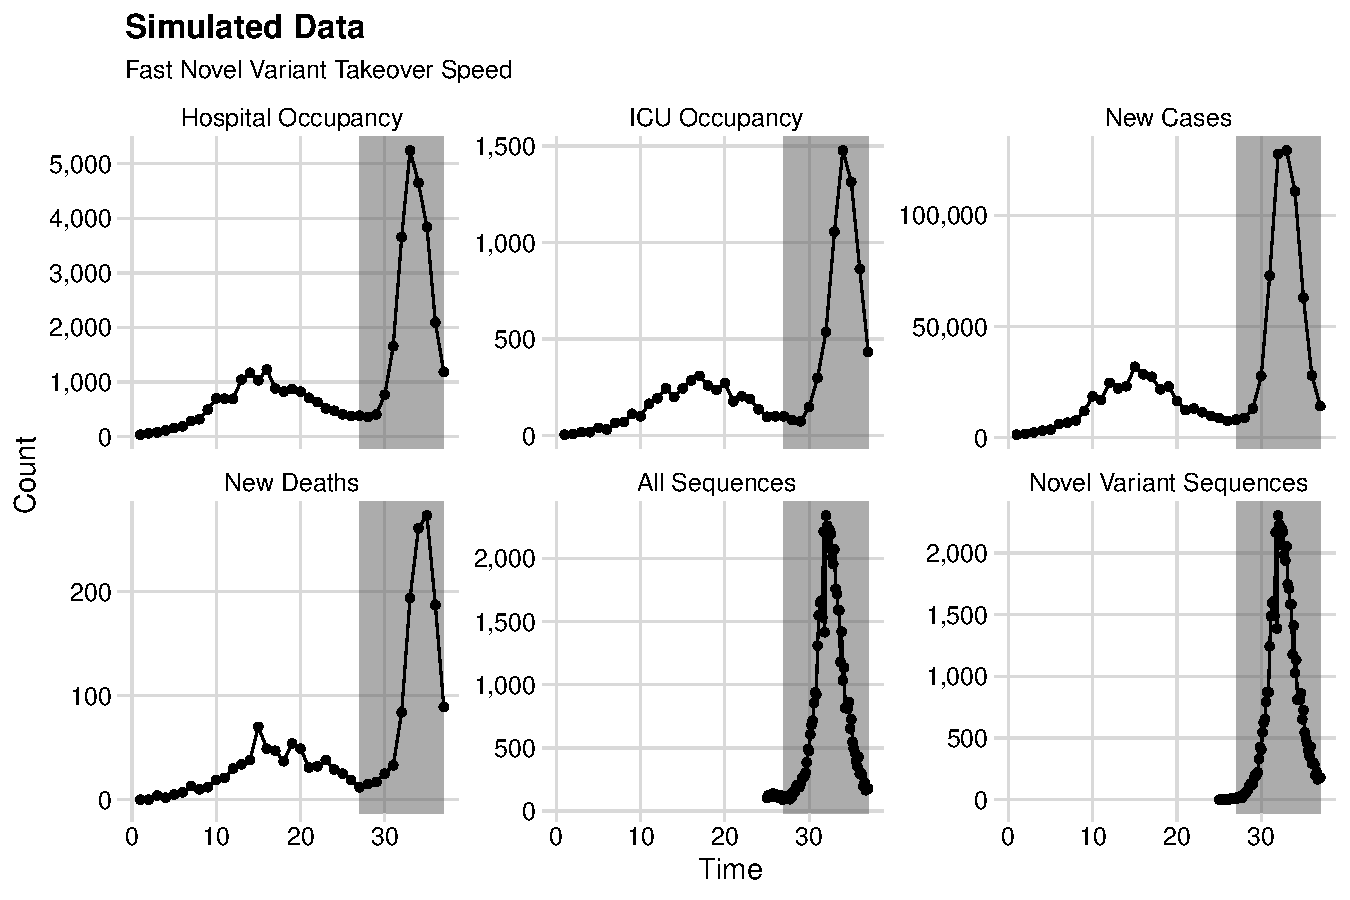
\includegraphics[width=1.0\columnwidth]{simulated_binned_data_fast_plot}
    \caption[Simulated data set for the fast takeover speed scenario.]{Simulated data set for the fast takeover speed scenario.
    The gray shaded areas indicate the time points for which we create forecasts}
    \label{ch_5:fig:simulated_binned_data_fast_plot}
\end{figure}


\section{Additional simulation study results}
\label{ch_5:sec:sim_cases_icu_death}


\begin{xltabular}{\columnwidth}{c>{\RaggedRight}Xllc}
\label{ch_5:tbl:simulation_prior_table}\\
\caption{TKTK}\\[\belowcaptionskip]
% (1) a model where \( R_0(t) \) is a priori modeled as a GMRF and \( 1 / \kappa(t) \) is constant
% (2) a model where \( R_0(t) \) is constant and \( 1 / \kappa(t) \) is a priori modeled as a GMRF, and
% (3) a model where \( R_0(t) \) is constant and \( 1 / \kappa(t) \) is a function of the proportion of infectious individuals infected with the novel variant shown in \eqref{ch_5:eqn:kappa_delta}.}
\thead{Parameter} & \thead{Interpretation} & \thead{Prior} & \thead{Prior Median\\ (95\% Interval)} & Models\\ \hline
\( \iota_0 \) & proportion of novel variant at \( t^* \) & Logit-Normal(-2.94, 0.25) & \makecell{0.0500 \\ (0.0194, 0.1230)} & 3    \\
\( \iota_1^* \) & time novel variant takes to grow from 1\% to 99\% of the infectious population (weeks) & Log-Normal(2.56, 0.16) & \makecell{13.00 \\ ( 5.94, 28.50)} & 3\\
\( 1 / \sqrt{\phi_W} \) & over-dispersion parameter for observed new cases & Half-Normal(0,1) & \makecell{0.6740 \\ (0.0313, 2.2400)} & 1,2,3\\
\( 1 / \sqrt{\phi_X} \) & over-dispersion parameter for observed hospital occupancy & Half-Normal(0,1) & \makecell{0.6740 \\ (0.0313, 2.2400)} & 1,2,3\\
\( 1 / \sqrt{\phi_Y} \) & over-dispersion parameter for observed ICU occupancy & Half-Normal(0,1) & \makecell{0.6740 \\ (0.0313, 2.2400)} & 1,2,3\\
\( 1 / \sqrt{\phi_Z} \) & over-dispersion parameter for observed new deaths & Half-Normal(0,1) & \makecell{0.6740 \\ (0.0313, 2.2400)} & 1,2,3\\
\( 1 / \sqrt{\phi_V} \) & over-dispersion parameter for observed new sequences of new variant & Half-Normal(0,1) & \makecell{0.6740 \\ (0.0313, 2.2400)} & 3\\
\( \zeta \) & time offset (weeks) for relationship between immunity duration \( 1 / \kappa(t) \) and proportion of novel variant \( \delta(t) \) & Log-Normal(0, 0.64) & \makecell{1.000 \\ (0.208, 4.800)} & 3 \\
\( 1 / \kappa \) & immunity duration & Log-Normal(3, 0.04) & \makecell{20.0 \\ (13.5, 29.6)} & 1 \\
\( \exp\left(1/\kappatilde_1\right) \) & initial immunity duration & Log-Normal(3, 0.04) & \makecell{20.0 \\ (13.5, 29.6)} & 2 \\
\( \sigma_\kappa \) & standard deviation for immunity duration GMRF & Log-Normal(-2, 0.01) & \makecell{0.135 \\ (0.111, 0.165)} & 2 \\
\( \exp \left( \alpha_0 \right)\) & maximum immunity duration & Log-Normal(3, 0.0025) & \makecell{20.0 \\ (18.1, 22.1)} & 3 \\
\( \alpha_2 \) & shape of transition from maximum immunity duration to minimum immunity duration & Log-Normal(0, 0.25) & \makecell{1.000 \\ (0.375, 2.660)} & 3 \\
\( \alpha_1^*  \) & proportion of maximum immunity duration that is minimum immunity duration & Logit-Normal(-1.1, 0.09) & \makecell{0.250 \\ (0.156, 0.375)} & 3 \\
\( \rho^W \) &  case detection rate & Logit-Normal(-1.39, 0.04) & \makecell{0.200 \\ (0.145, 0.270)} & 1,2,3 \\
\( R_0 \) & basic reproduction number & Log-Normal(0.405, 0.04) & \makecell{1.50 \\ (1.01, 2.22)} & 2,3 \\
\( \exp \left( \tilde{R}_{0,1} \right) \) & initial basic reproduction number & Log-Normal(0.405, 0.04) & \makecell{1.50 \\ (1.01, 2.22)} & 1 \\
\( \sigma_{R_0} \) & standard deviation for basic reproduction number GMRF & Log-Normal(-2, 0.01) & \makecell{0.135 \\ (0.111, 0.165)} & 1\\
\( 1 / \gamma \) & mean latent period duration (weeks) & Log-Normal(-1.25, 0.04) & \makecell{0.286 \\ (0.193, 0.423)} & 1,2,3 \\
\( 1 / \nu \) & Mean infectious period duration (weeks) & Log-Normal(-0.336, 0.04) & \makecell{0.714 \\ (0.483, 1.060)} & 1,2,3\\
\( 1 / \eta \) & mean hospitalization duration (weeks) & Log-Normal(-0.847, 0.04) & \makecell{0.429 \\ (0.290, 0.634)} & 1,2,3\\
\( 1 / \omega \) & mean ICU stay duration (weeks) & Log-Normal(-0.336, 0.04) & \makecell{0.714 \\ (0.483, 1.060)} & 1,2,3\\
\( \tau \) & Infection-hospitalization ratio & Logit-Normal(-3.89, 0.04) & \makecell{0.0200 \\ (0.0136, 0.0293)} & 1,2,3 \\
\( \upsilon \) & Hospitalization-ICU admission ratio & Logit-Normal(-1.73, 0.04) & \makecell{0.150 \\ (0.107, 0.207)} & 1,2,3 \\
\( \chi \) & ICU-fatality ratio & Logit-Normal(-1.73, 0.04) & \makecell{0.150 \\ (0.107, 0.207)} & 1,2,3 \\
\( \rho^Z \) & death detection rate & Logit-Normal(2.2, 0.04) & \makecell{0.900 \\ (0.859, 0.930)} & 1,2,3 \\
\( E\left(0\right) \) & Initial proportion of infected, but not yet infectious population & Logit-Normal(-8.52, 0.04) & \makecell{0.000200 \\ (0.000135, 0.000296)} & 1,2,3 \\
\( I\left(0\right) \) & Initial proportion of infectious population & Logit-Normal(-7.82, 0.04) & \makecell{0.000400 \\ (0.000270, 0.000592)} & 1,2,3 \\
\( R\left(0\right) \) & Initial proportion of immune population & Logit-Normal(-1.39, 0.16) & \makecell{0.200 \\ (0.102, 0.354)} & 1,2,3
\end{xltabular}

% ONLY REAL DATA double check the values are correct
% \operatorname{logistic}\left(\rhowtilde_1\right) & initial case detection rate & Logit-Normal(-1.39, 0.04) & \makecell{0.200 \\ (0.145, 0.270)} & 1,2,3\\
% \( \sigma_{\rho^Y} \) & standard deviation for case detection rate GMRF & Log-Normal(-2, 0.01) & \makecell{0.135 \\ (0.111, 0.165)} & 1,2,3 \\
\begin{figure}
    \centering
    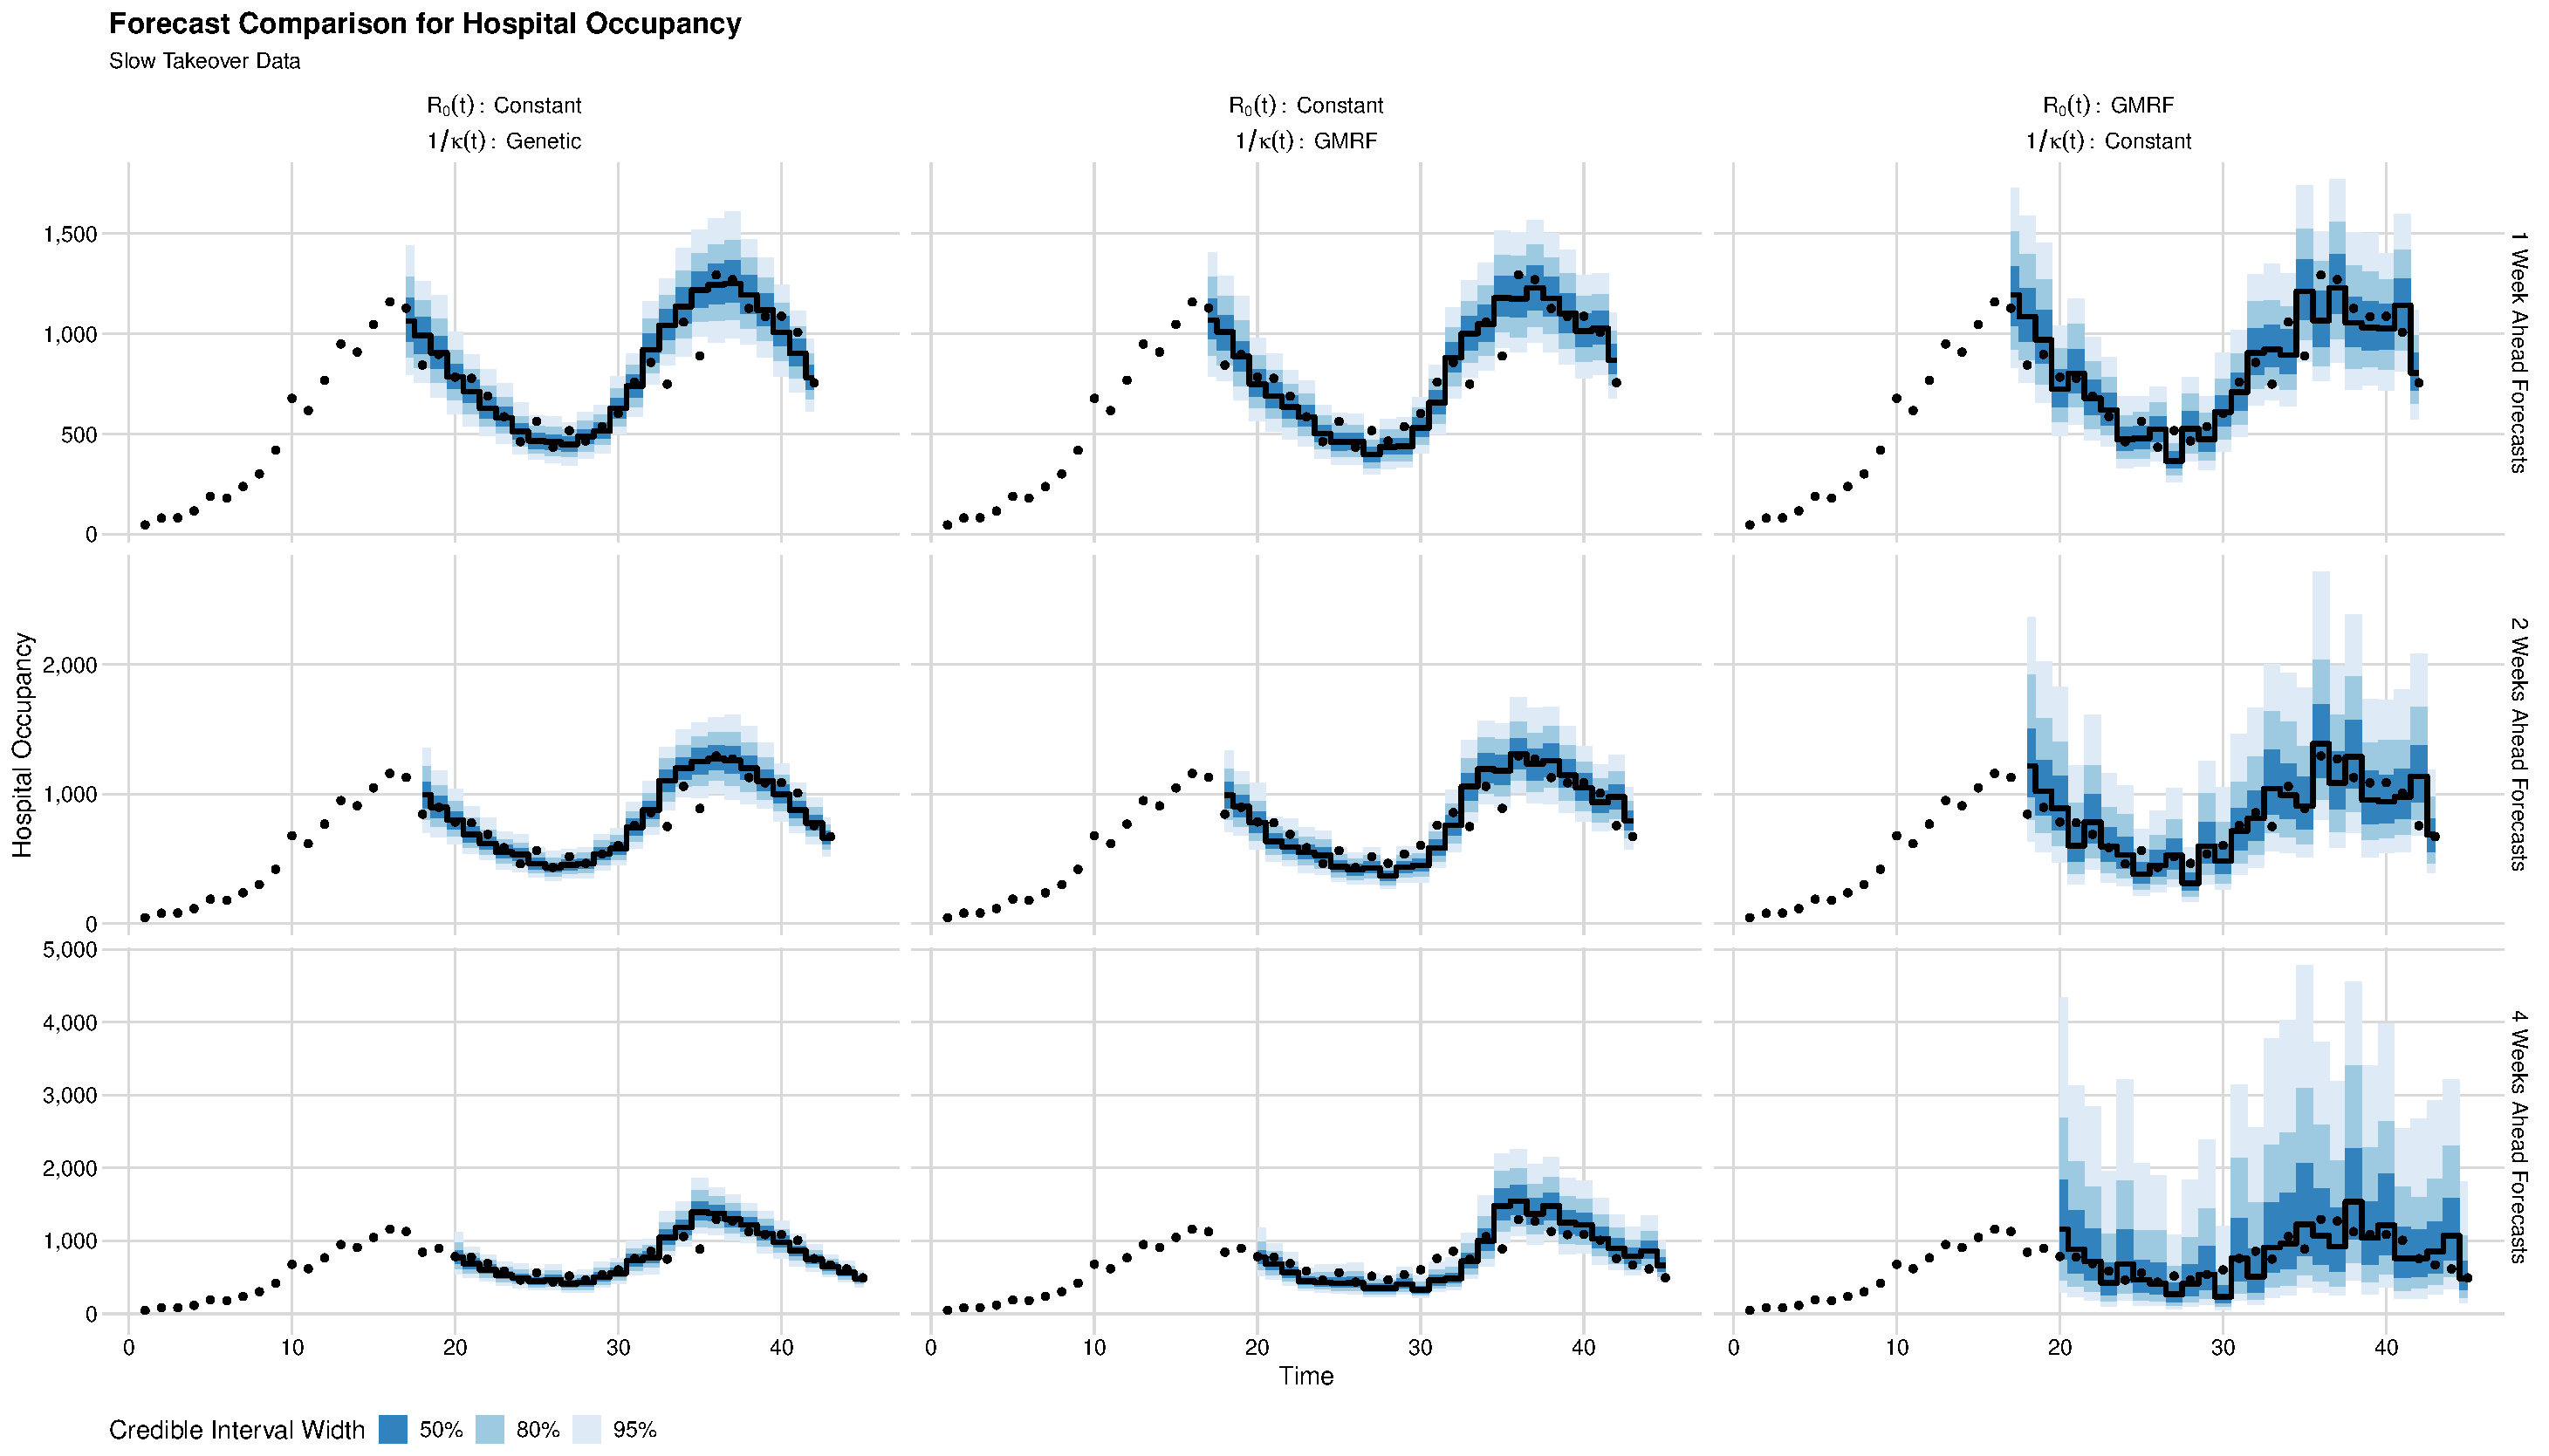
\includegraphics[width=1.0\columnwidth]{simulated_forecast_comparison_data_hospitalizations_slow_plot}
\caption[Hospital occupancy forecasts for simulated slow takeover speed data.]{Hospital occupancy forecasts from three models at 1, 2, and 4-week forecast horizons for the simulated slow takeover speed data.}
    \label{ch_5:fig:simulated_forecast_comparison_data_hospitalizations_slow_plot}
\end{figure}

\begin{figure}
    \centering
    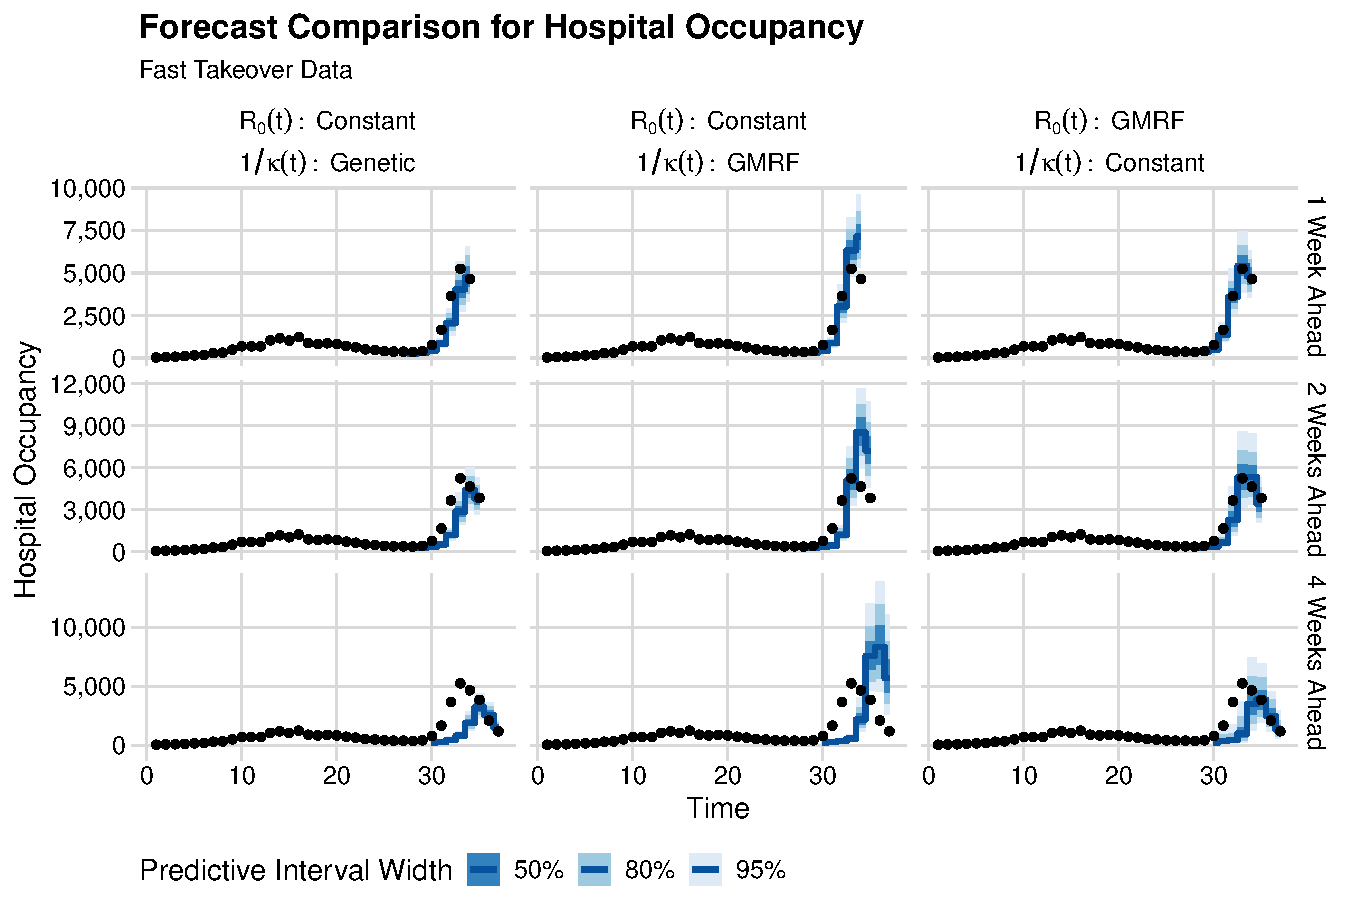
\includegraphics[width=1.0\columnwidth]{simulated_forecast_comparison_data_hospitalizations_fast_plot}
\caption[Hospital occupancy forecasts for simulated fast takeover speed data.]{Hospital occupancy forecasts from three models at 1, 2, and 4-week forecast horizons for the simulated fast takeover speed data.}
    \label{ch_5:fig:simulated_forecast_comparison_data_hospitalizations_fast_plot}
\end{figure}

\begin{figure}
    \centering
    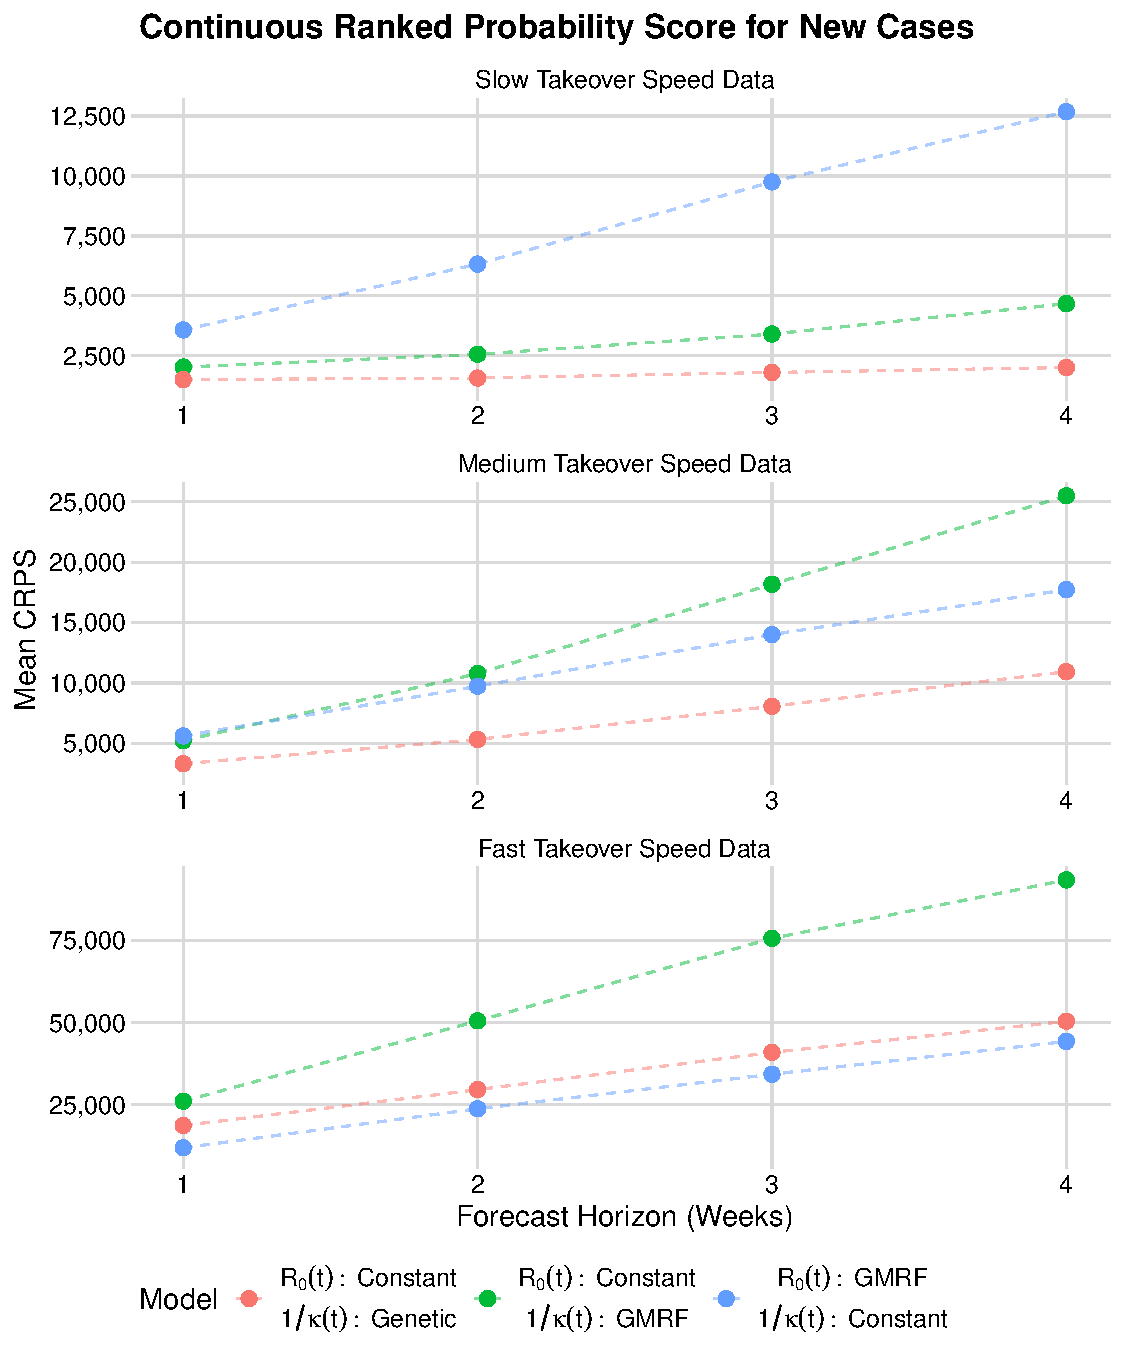
\includegraphics[width=1.0\columnwidth]{simulated_crps_comparison_dotplot_data_new_cases_plot}
    \caption{CRPS summaries for new cases forecasts at 1, 2, and 4-week horizons for three simulated data sets. Lower CRPS is better.}
    \label{ch_5:fig:simulated_crps_comparison_dotplot_data_new_cases_plot}
\end{figure}

\begin{figure}
    \centering
    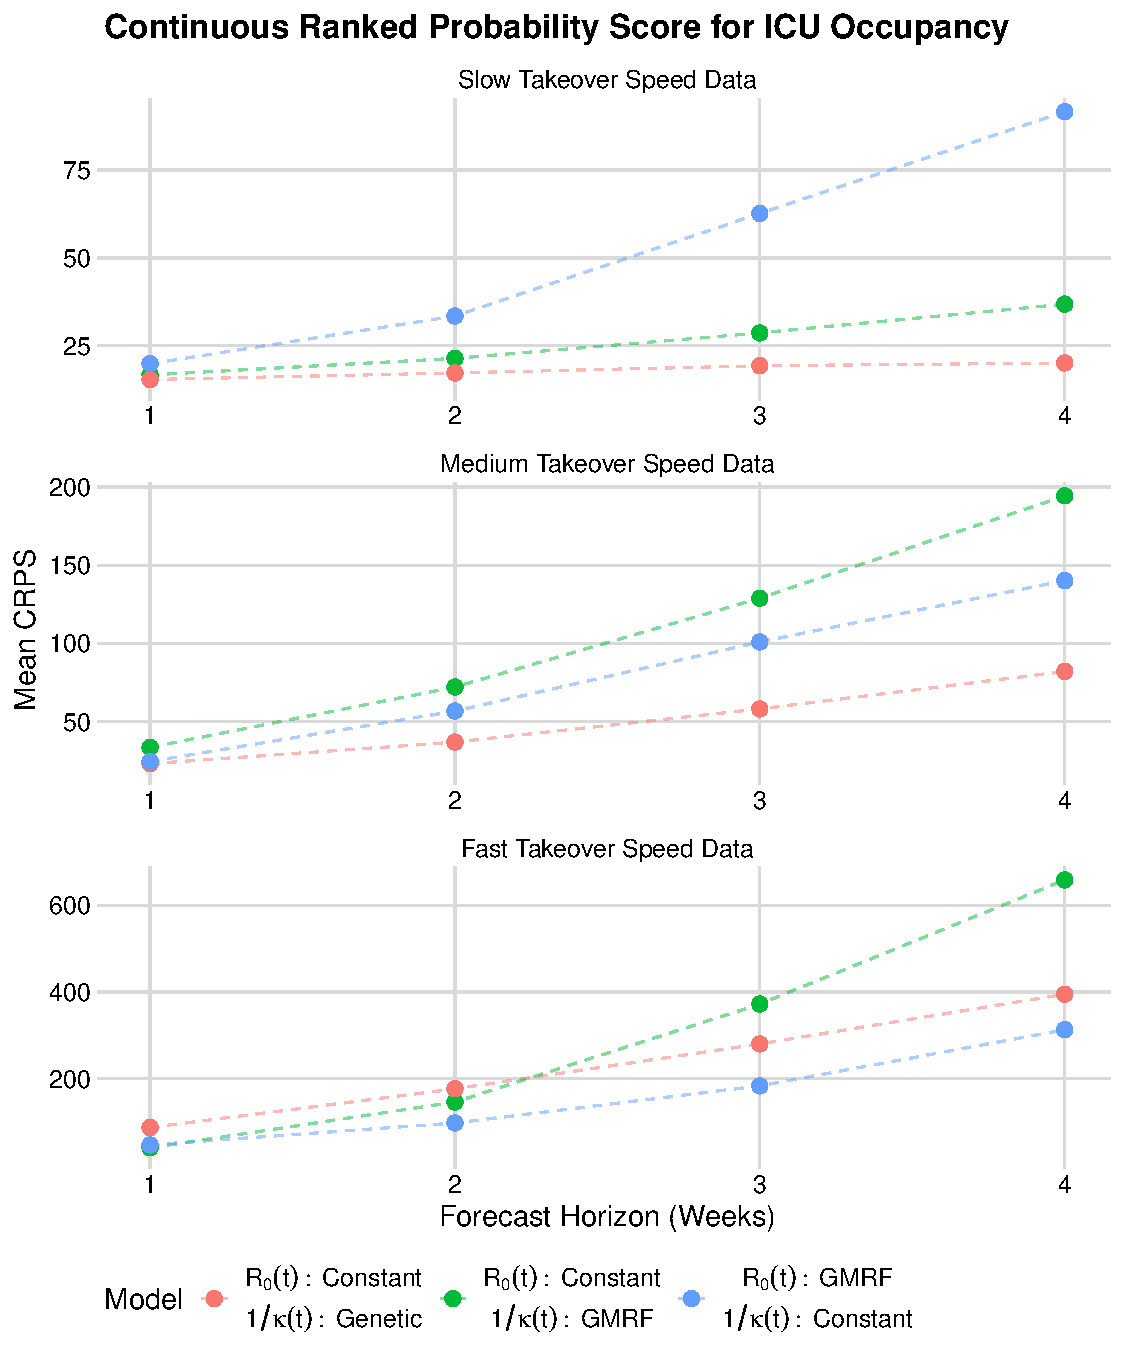
\includegraphics[width=1.0\columnwidth]{simulated_crps_comparison_dotplot_data_icu_plot}
    \caption{CRPS summaries for ICU occupancy forecasts at 1, 2, and 4-week horizons for three simulated data sets. Lower CRPS is better.}
    \label{ch_5:fig:simulated_crps_comparison_dotplot_data_icu_plot}
\end{figure}

\begin{figure}
    \centering
    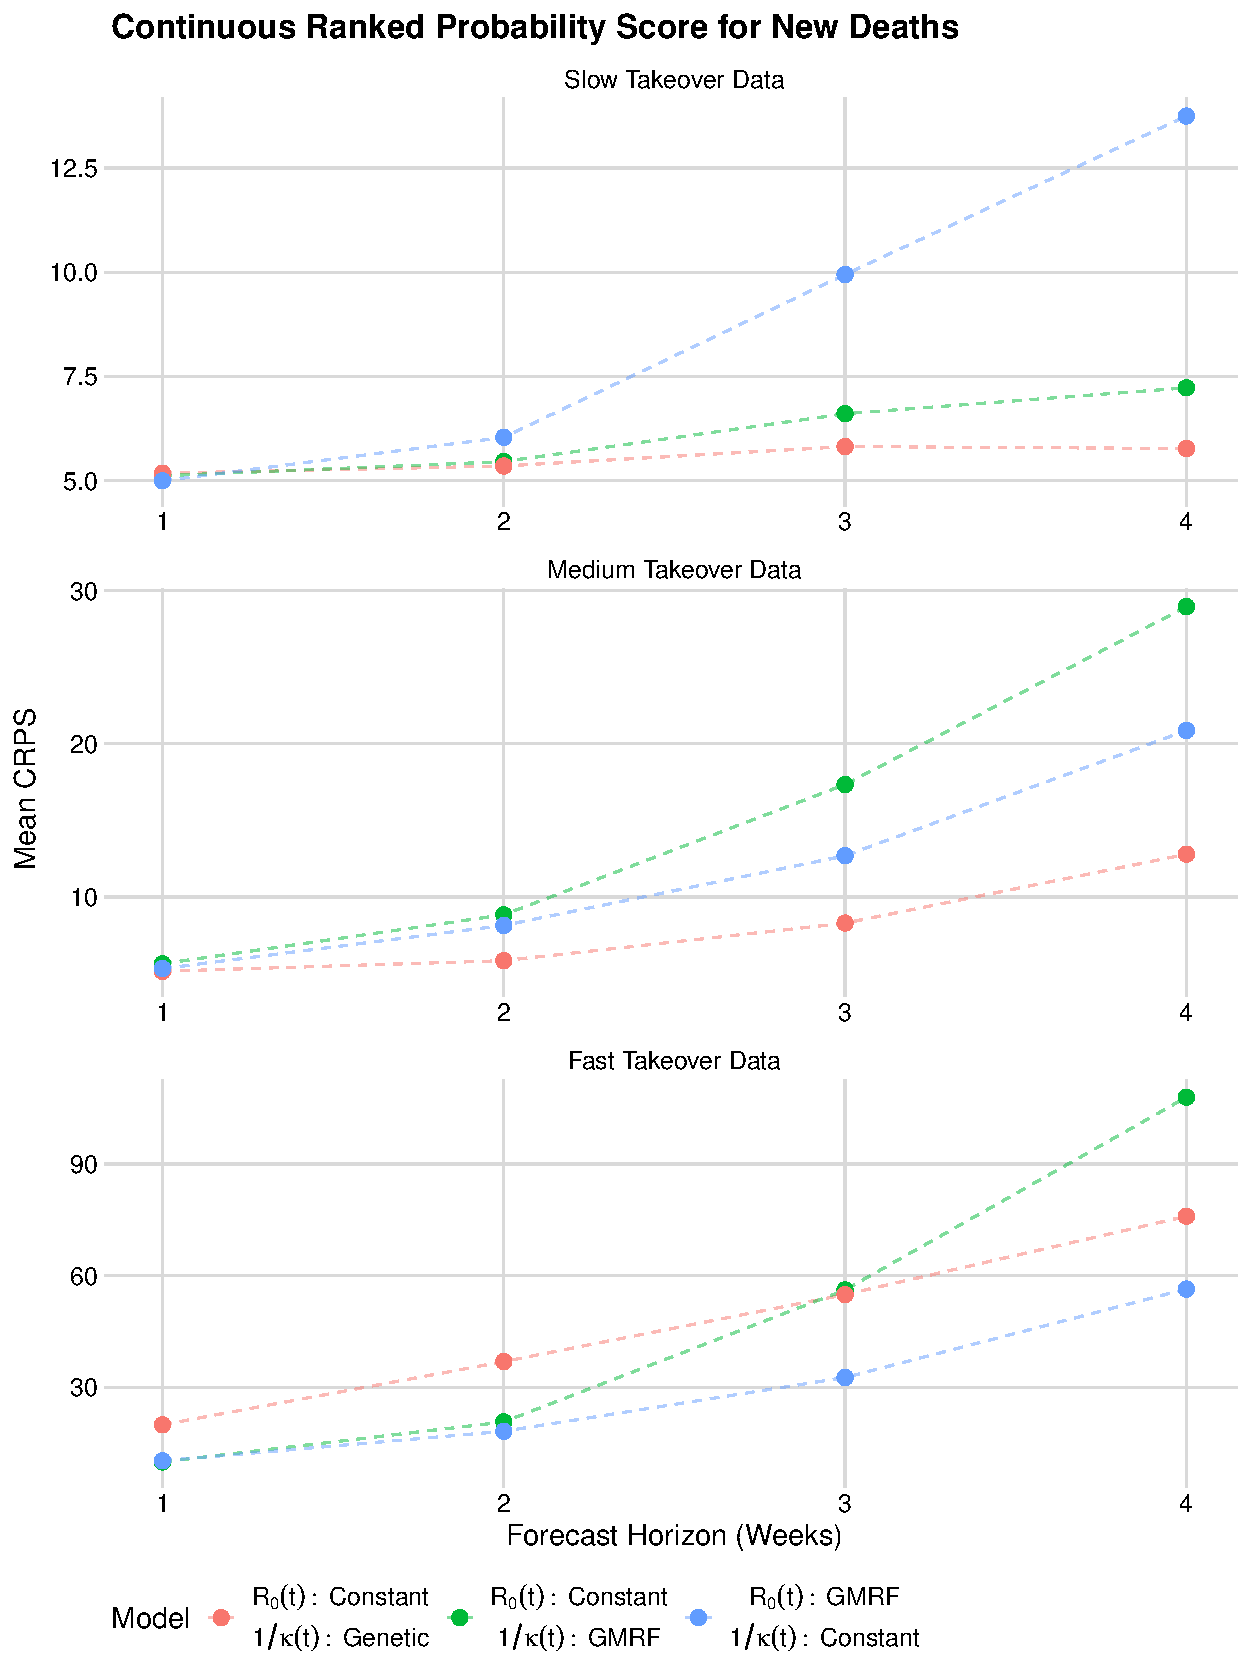
\includegraphics[width=1.0\columnwidth]{simulated_crps_comparison_dotplot_data_new_deaths_plot}
    \caption{CRPS summaries for new deaths forecasts at 1, 2, and 4-week horizons for three simulated data sets. Lower CRPS is better.}
    \label{ch_5:fig:simulated_crps_comparison_dotplot_data_new_deaths_plot}
\end{figure}

\begin{figure}
    \centering
    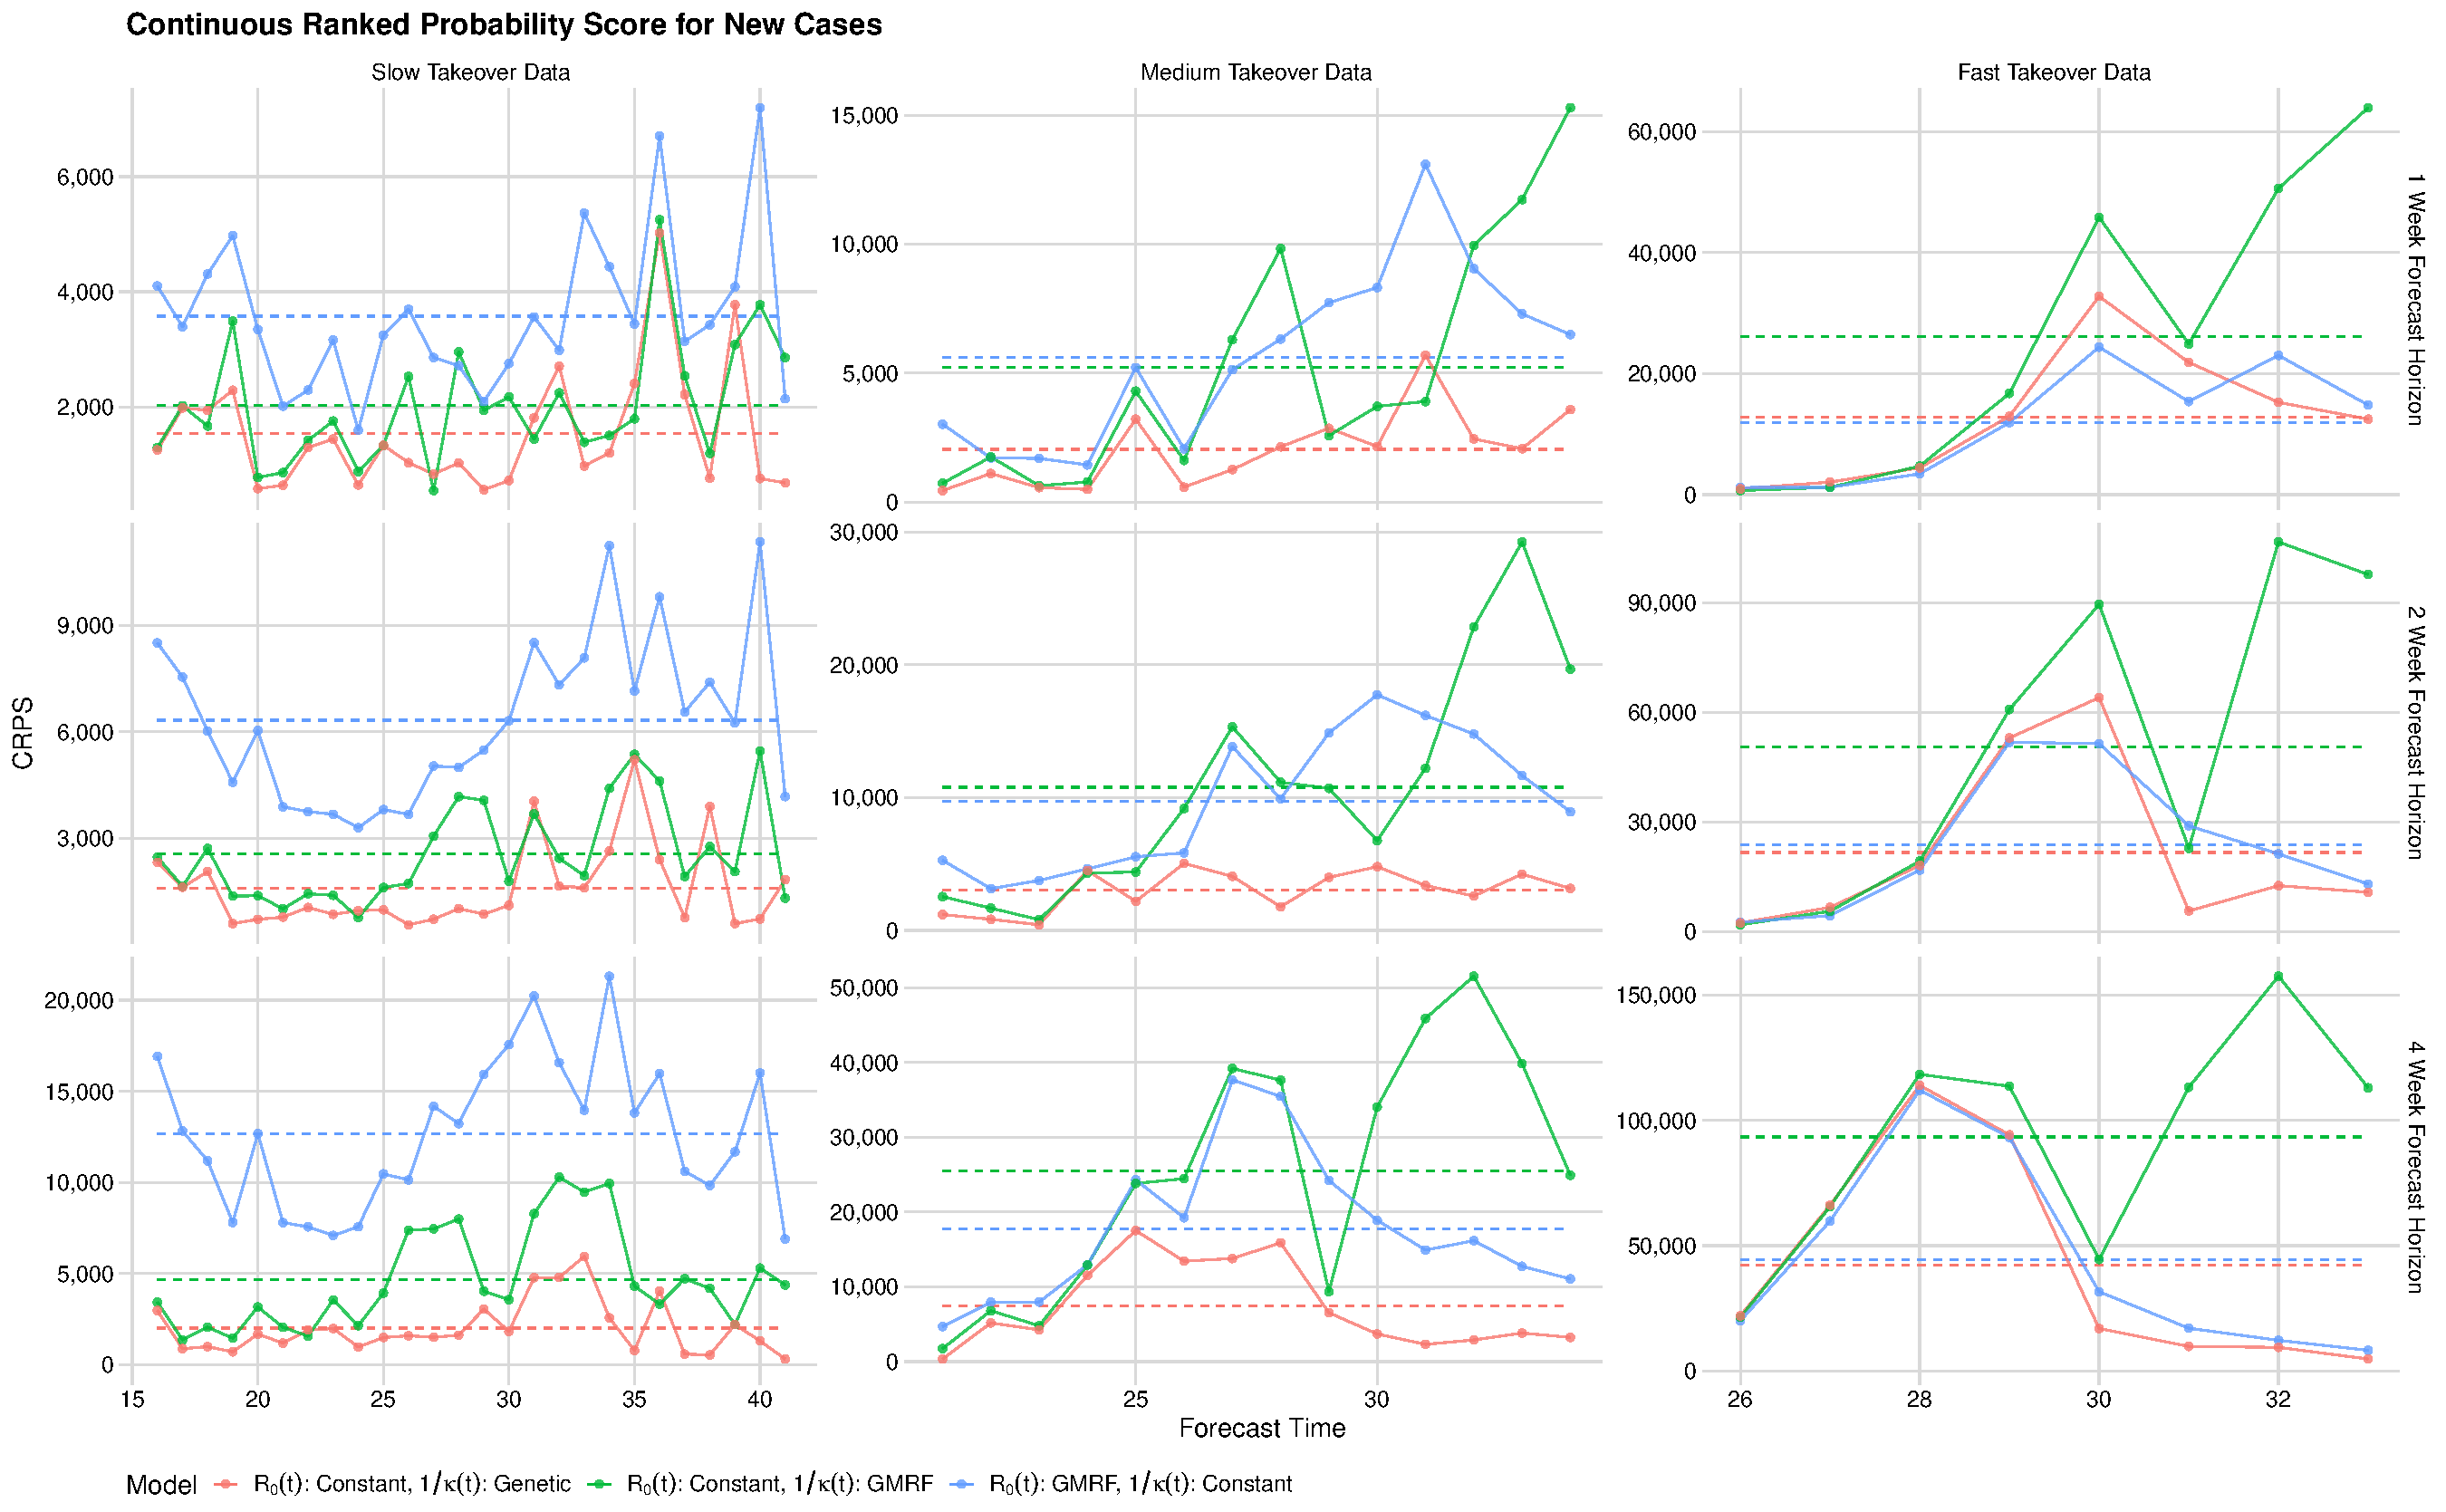
\includegraphics[width=1.0\columnwidth]{simulated_crps_comparison_data_new_cases_plot}
    \caption{Individual CRPS for new cases forecasts at 1, 2, and 4-week horizons for three simulated data sets. Lower CRPS is better.}
    \label{ch_5:fig:simulated_crps_comparison_data_new_cases_plot}
\end{figure}

\begin{figure}
    \centering
    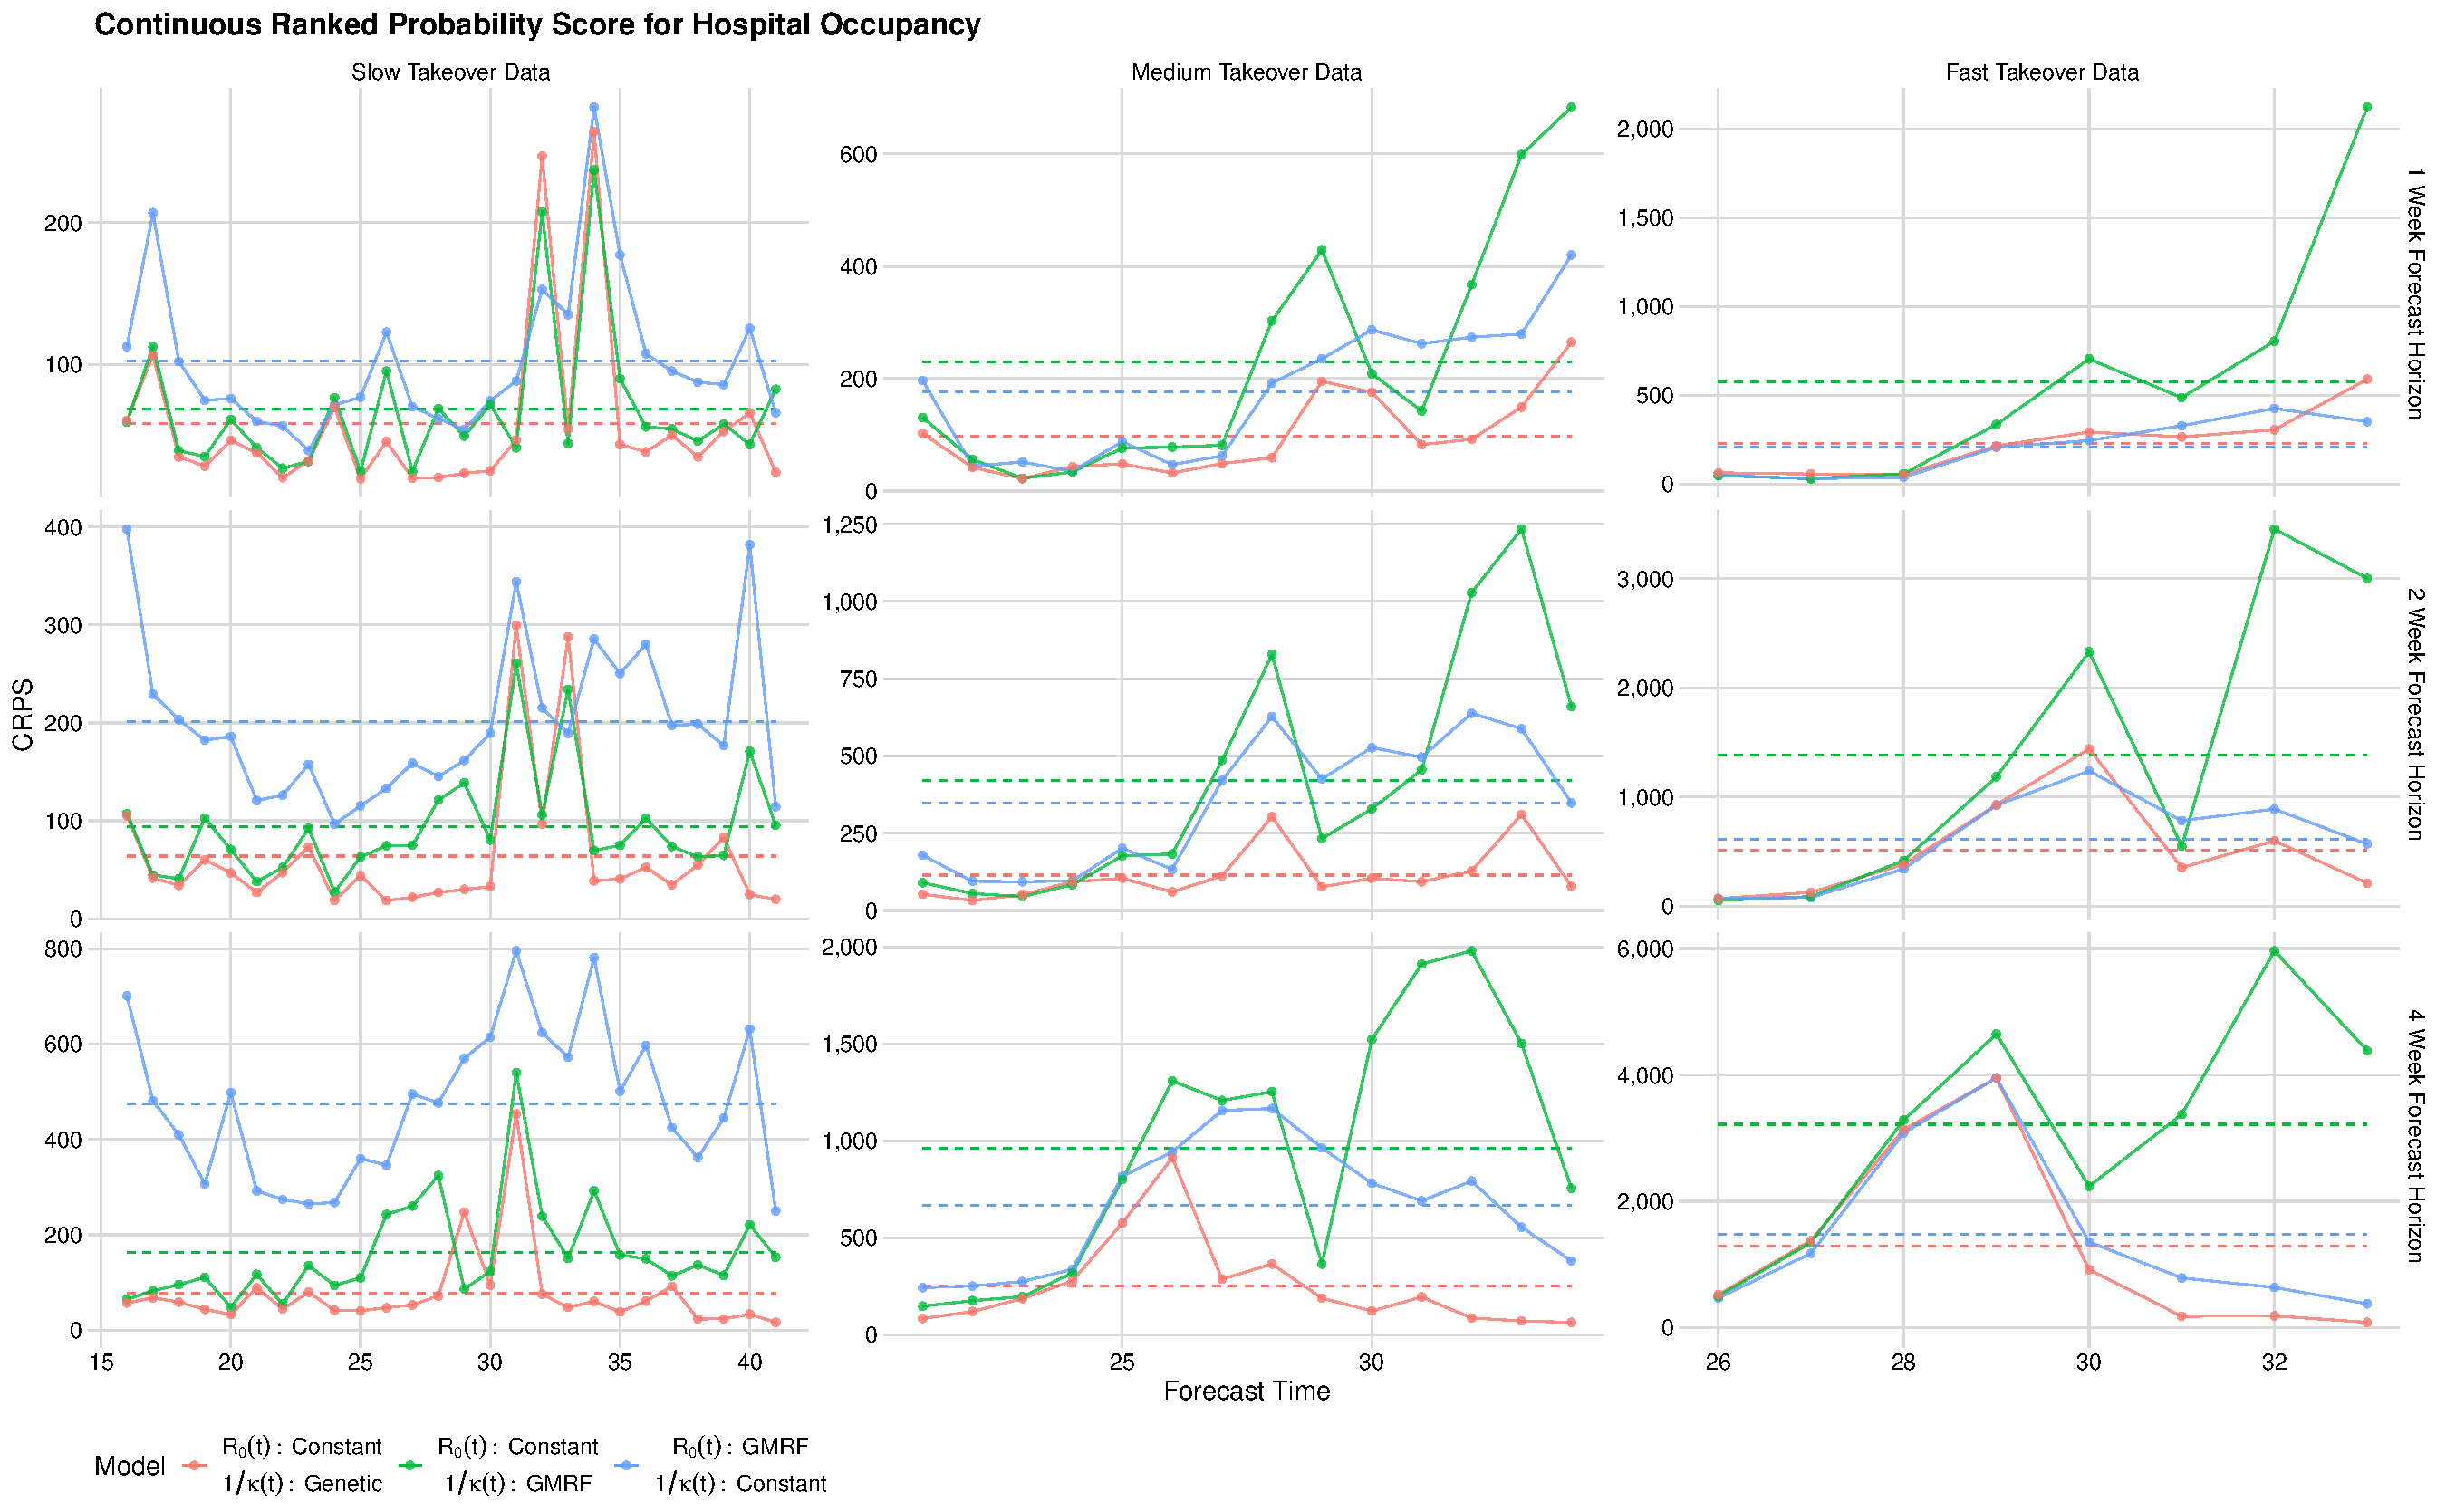
\includegraphics[width=1.0\columnwidth]{simulated_crps_comparison_data_hospitalizations_plot}
    \caption{Individual CRPS for hospital occupancy forecasts at 1, 2, and 4-week horizons for three simulated data sets. Lower CRPS is better.}
    \label{ch_5:fig:simulated_crps_comparison_data_hospitalizations_plot}
\end{figure}

\begin{figure}
    \centering
    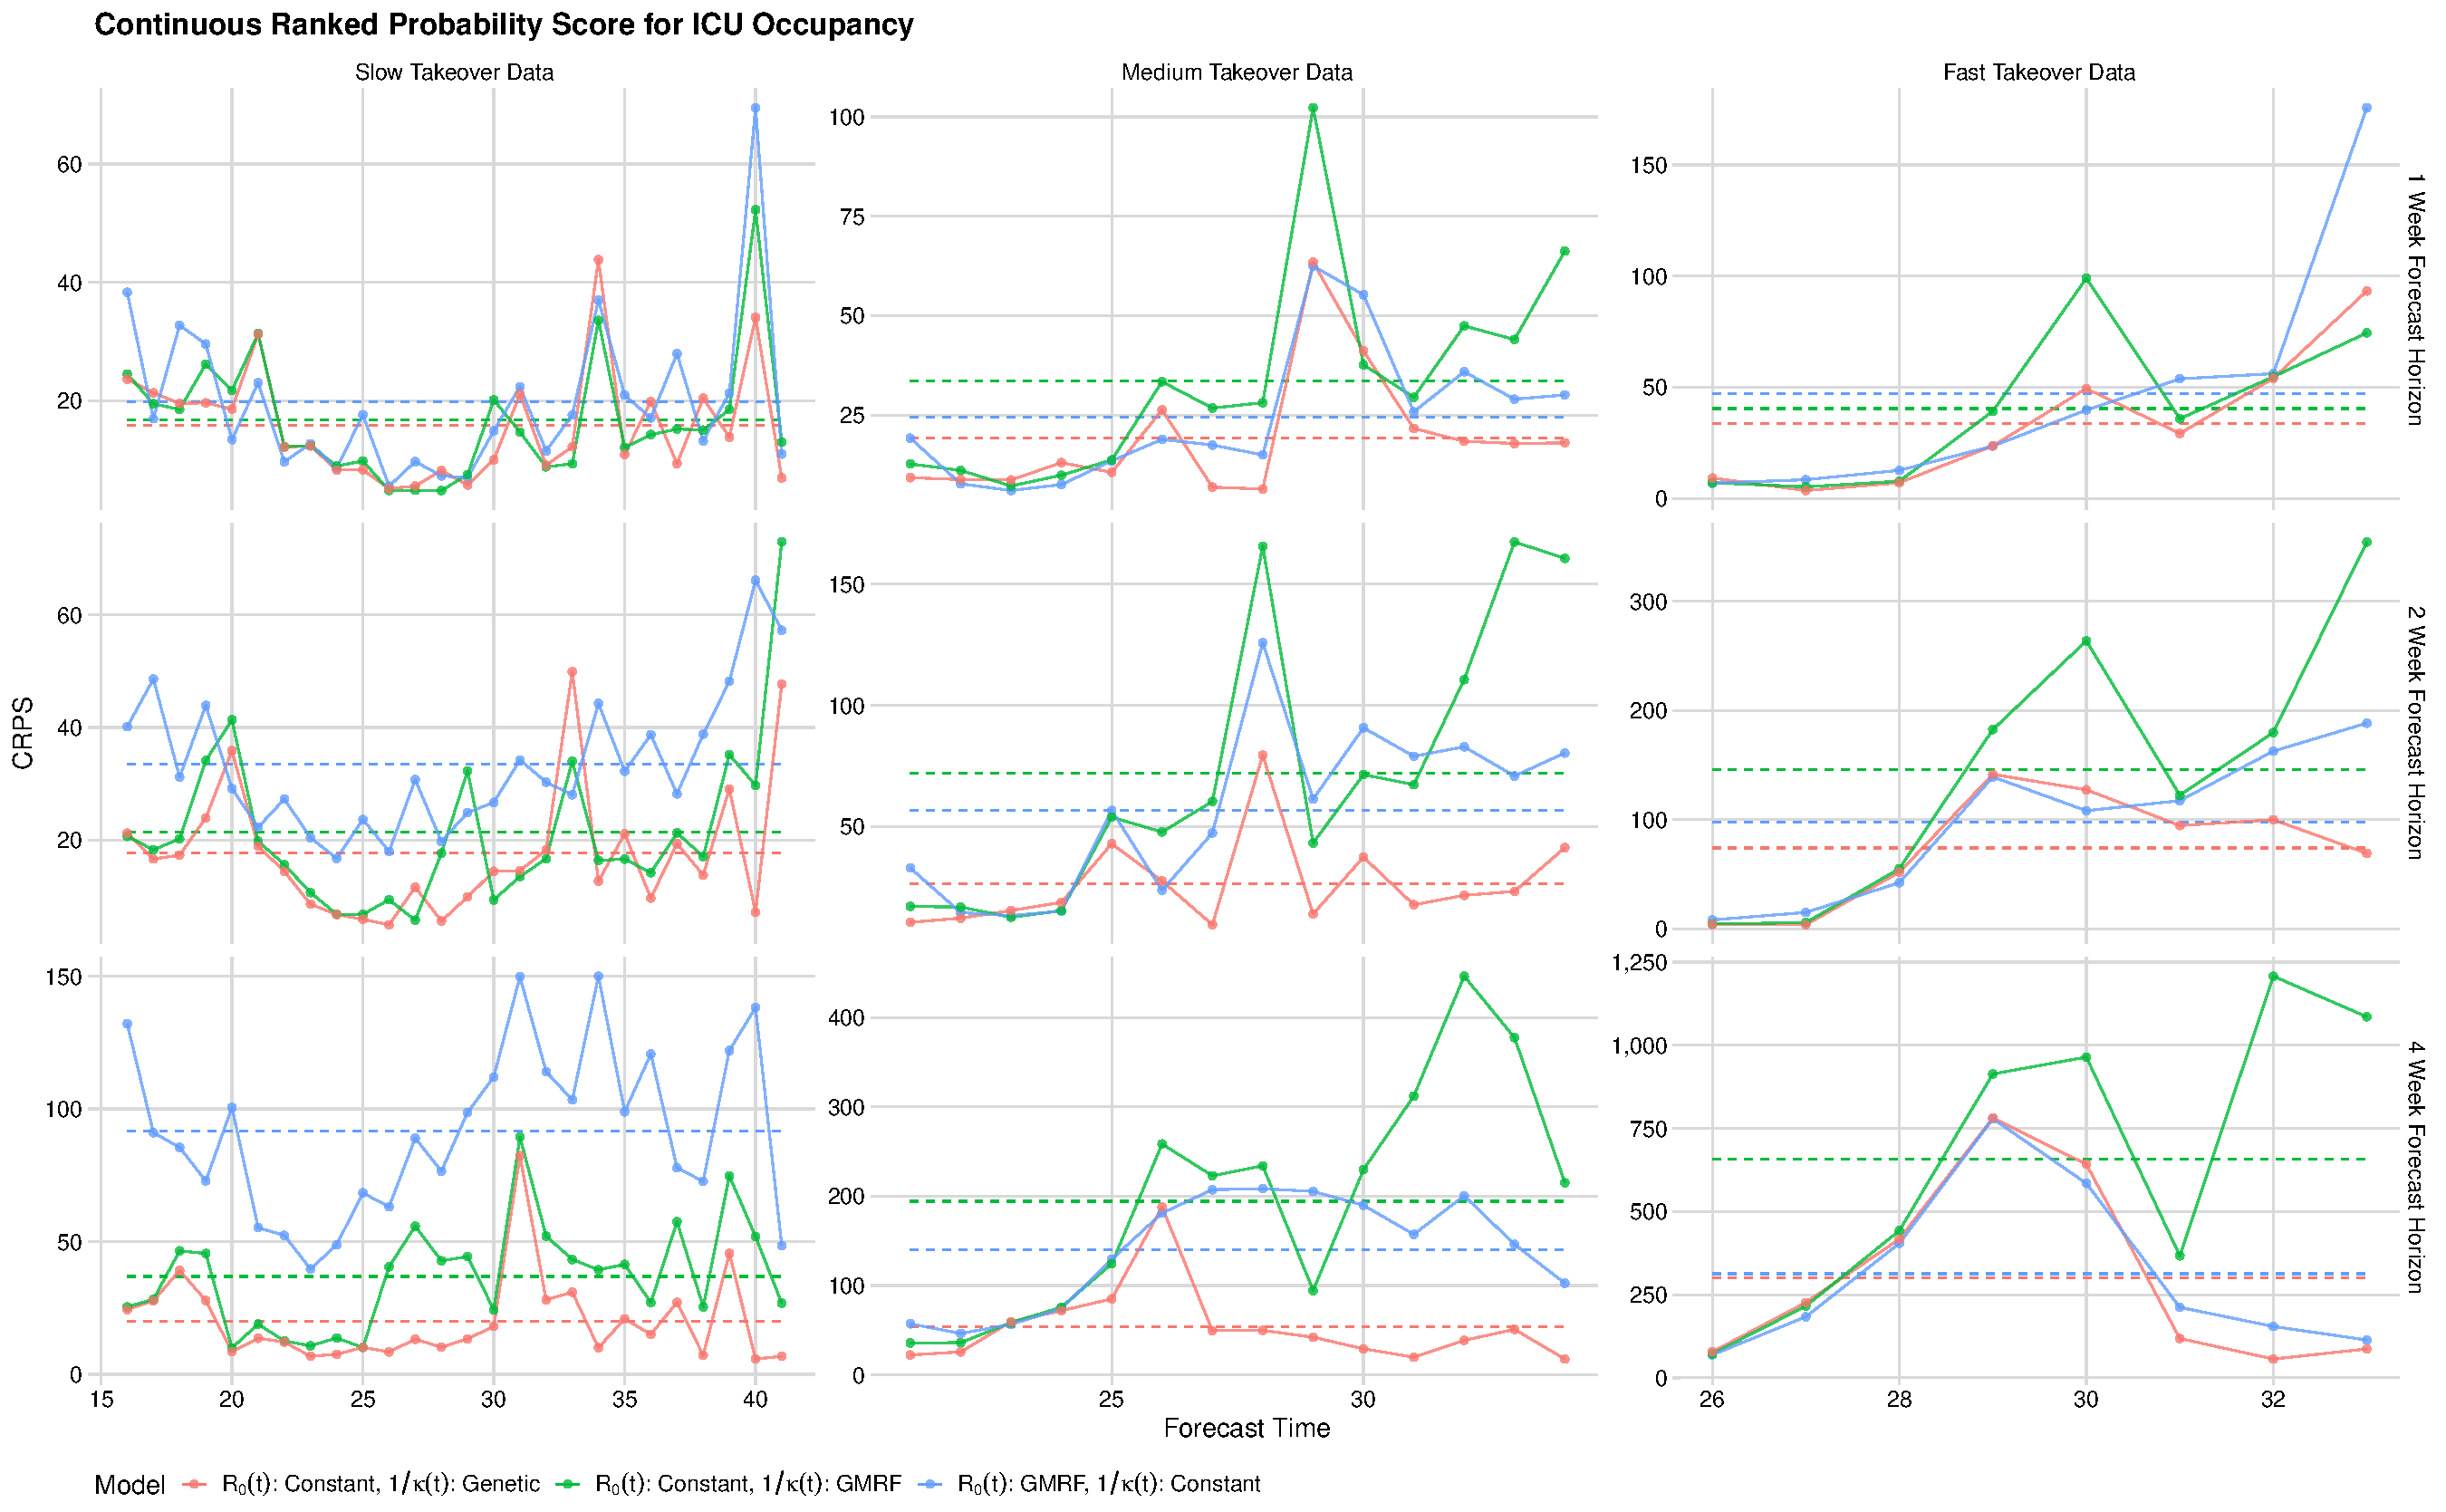
\includegraphics[width=1.0\columnwidth]{simulated_crps_comparison_data_icu_plot}
    \caption{Individual CRPS for ICU occupancy forecasts at 1, 2, and 4-week horizons for three simulated data sets. Lower CRPS is better.}
    \label{ch_5:fig:simulated_crps_comparison_data_icu_plot}
\end{figure}

\begin{figure}
    \centering
    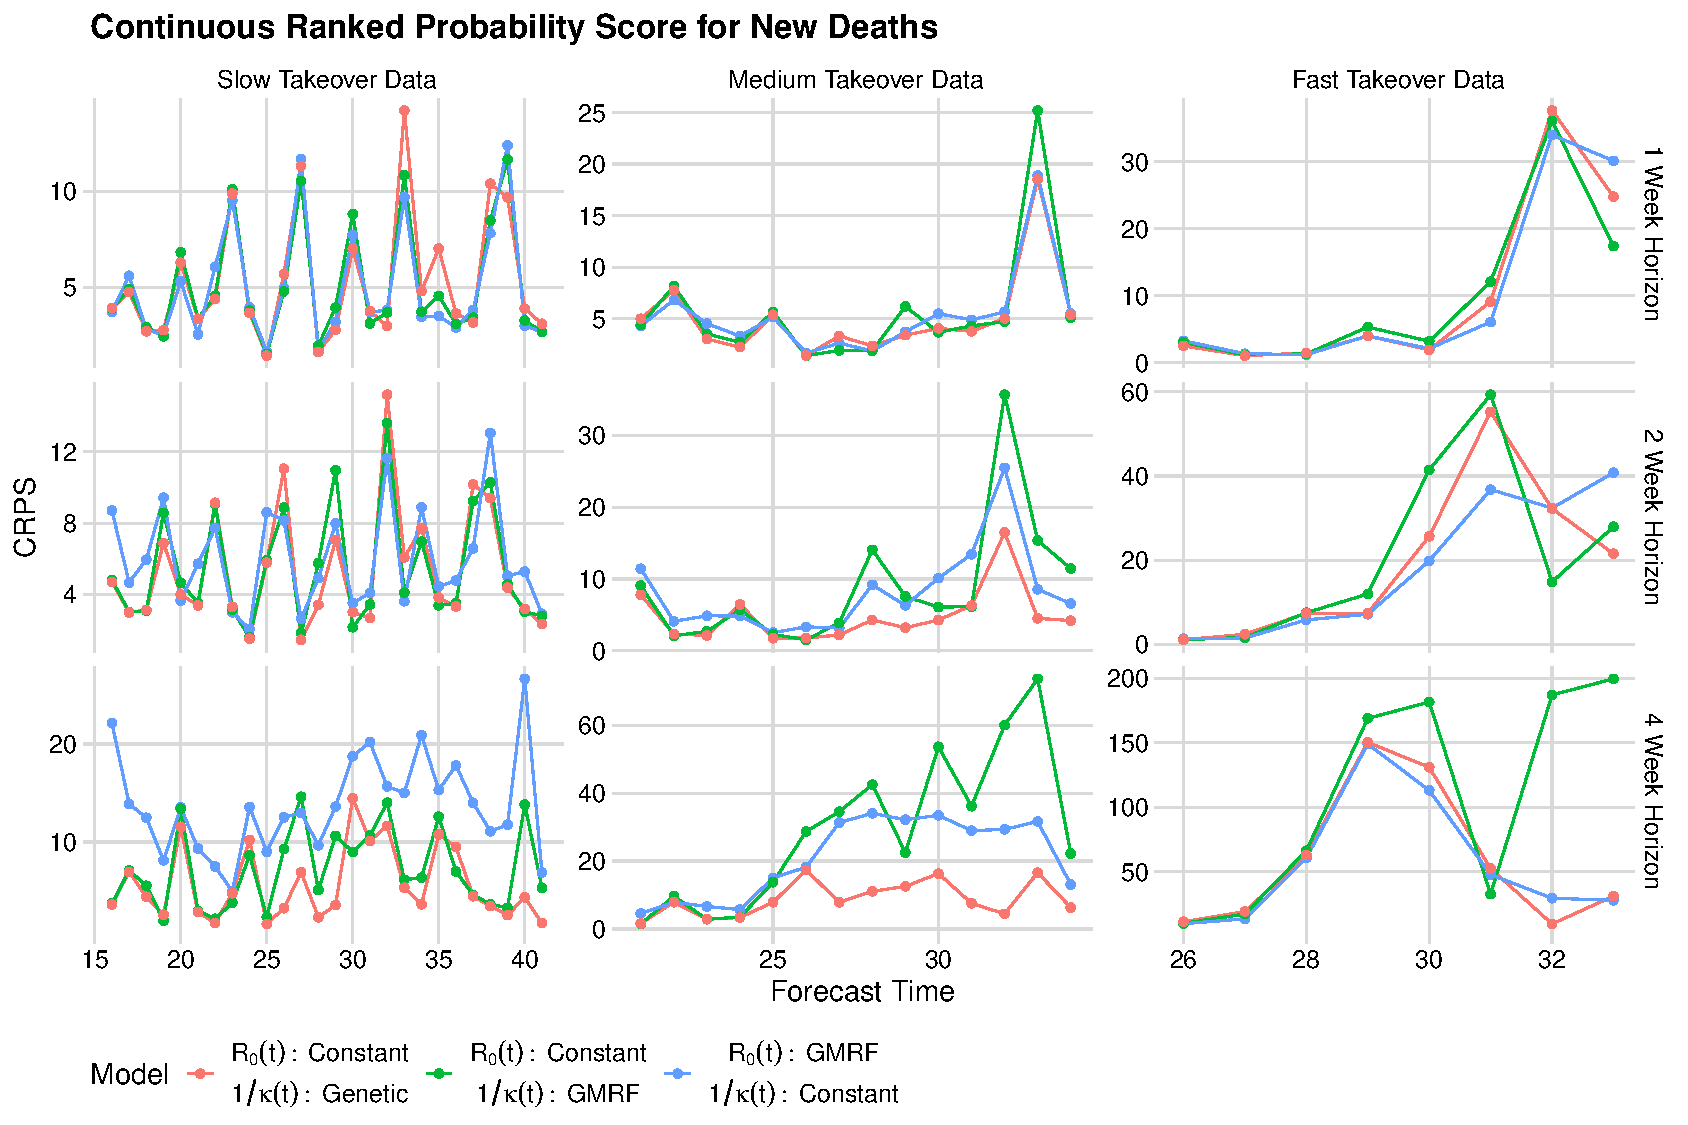
\includegraphics[width=1.0\columnwidth]{simulated_crps_comparison_data_new_deaths_plot}
    \caption{Individual CRPS for new deaths forecasts at 1, 2, and 4-week horizons for three simulated data sets. Lower CRPS is better.}
    \label{ch_5:fig:simulated_crps_comparison_data_new_deaths_plot}
\end{figure}

\begin{figure}
    \centering
    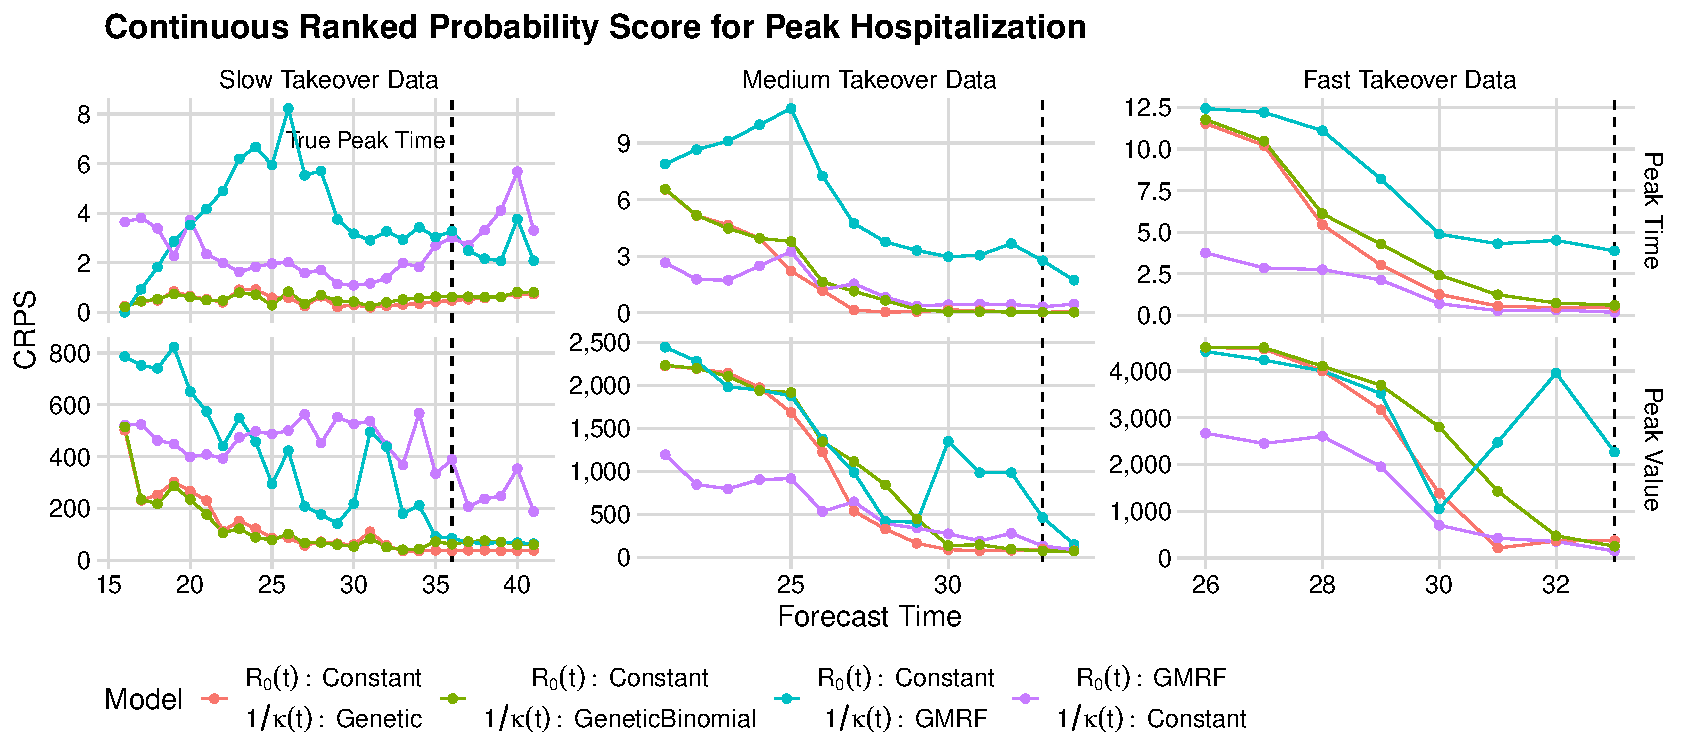
\includegraphics[width=1.0\columnwidth]{simulated_peak_crps_plot}
    \caption{Caption}
    \label{ch_5:fig:simulated_peak_crps_plot}
\end{figure}

\section{Simulation study sensitivity analysis}
\label{ch_5:sec:sim_sensitivity}

\begin{xltabular}{\columnwidth}{c>{\RaggedRight}Xllc}
    \label{ch_5:tbl:simulation_prior_sensitivity_table}\\
\caption{TKTK}\\[\belowcaptionskip]
	\thead{Parameter} & \thead{Interpretation} & \thead{Prior} & \thead{Prior Median\\ (95\% Interval)} \\ \hline
\end{xltabular}

\begin{figure}
    \centering
    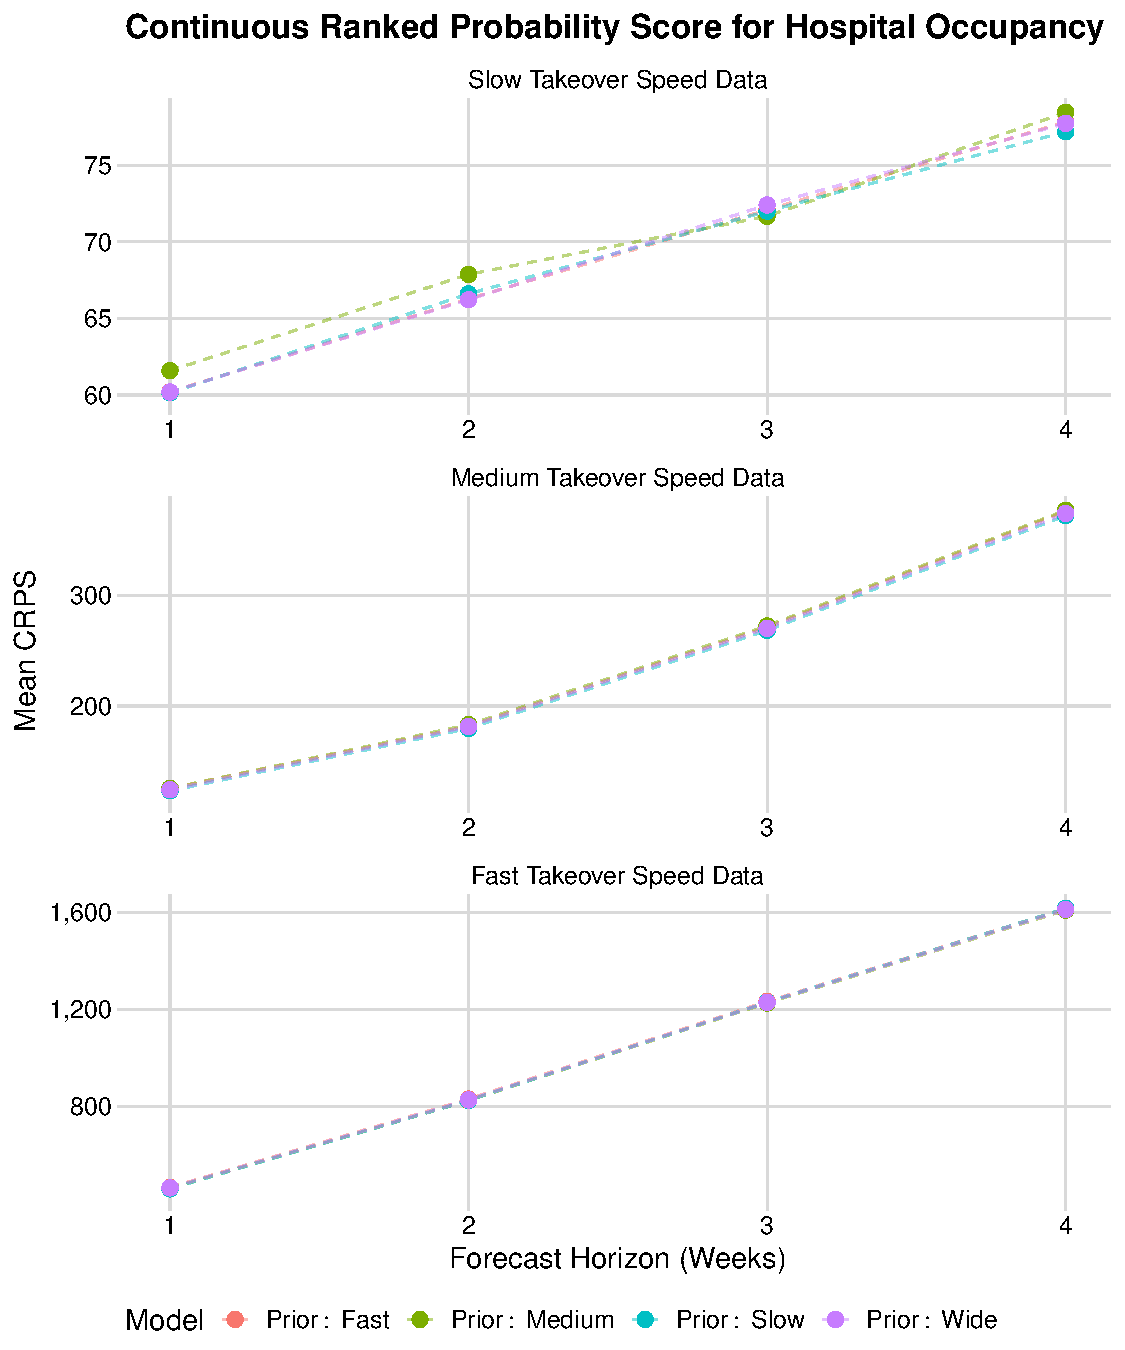
\includegraphics[width=0.75\columnwidth]{sensitivity_simulated_crps_comparison_dotplot_data_hospitalizations_plot}
    \caption[CRPS summaries for hospital occupancy forecasts for simulated data sets.]{CRPS summaries for hospital occupancy forecasts at 1, 2, and 4-week horizons for three simulated data sets. Lower CRPS is better.}
    \label{ch_5:fig:sensitivity_simulated_crps_comparison_dotplot_data_hospitalizations_plot}
\end{figure}


\begin{figure}
    \centering
    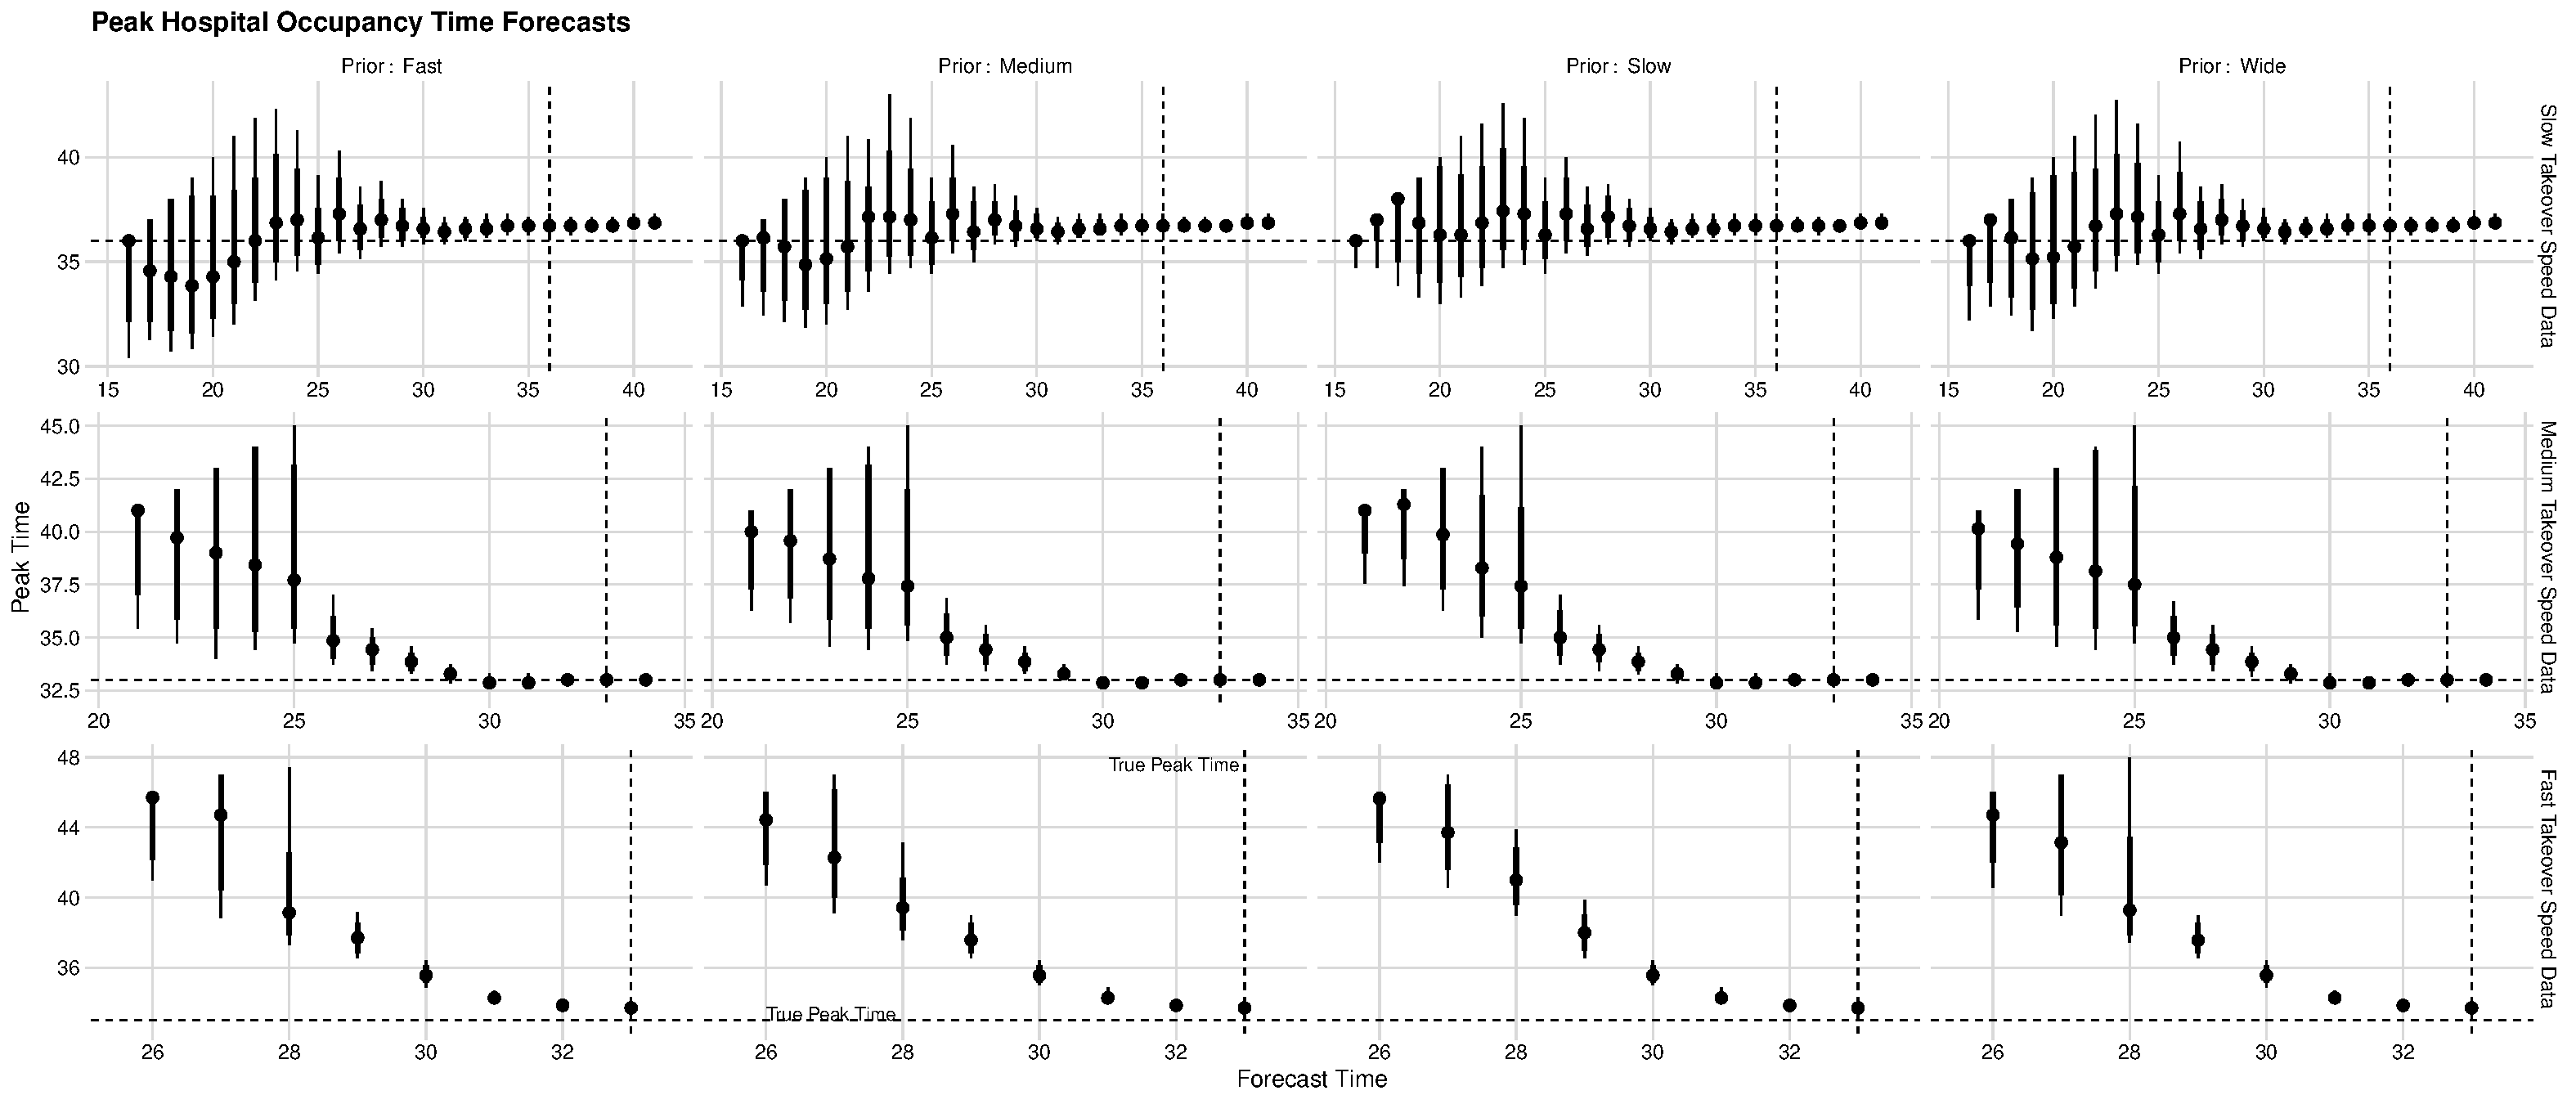
\includegraphics[width=1.0\columnwidth]{sensitivity_simulated_peak_assessment_time_plot}
    \caption[Posterior predictive intervals for peak hospital occupancy timing for simulated data sets.]{Posterior predictive intervals for the time at which hospital occupancy reaches its maximum in three simulated data sets.
    Dots indicate the median of the predictive distribution, while the thick and thin lines represent central 80\% and 95\% intervals, respectively.
    Horizontal and vertical dashed lines indicate the true peak hospitalization time.}
    \label{ch_5:fig:sensitivity_simulated_peak_assessment_time_plot}
\end{figure}

\begin{figure}
    \centering
    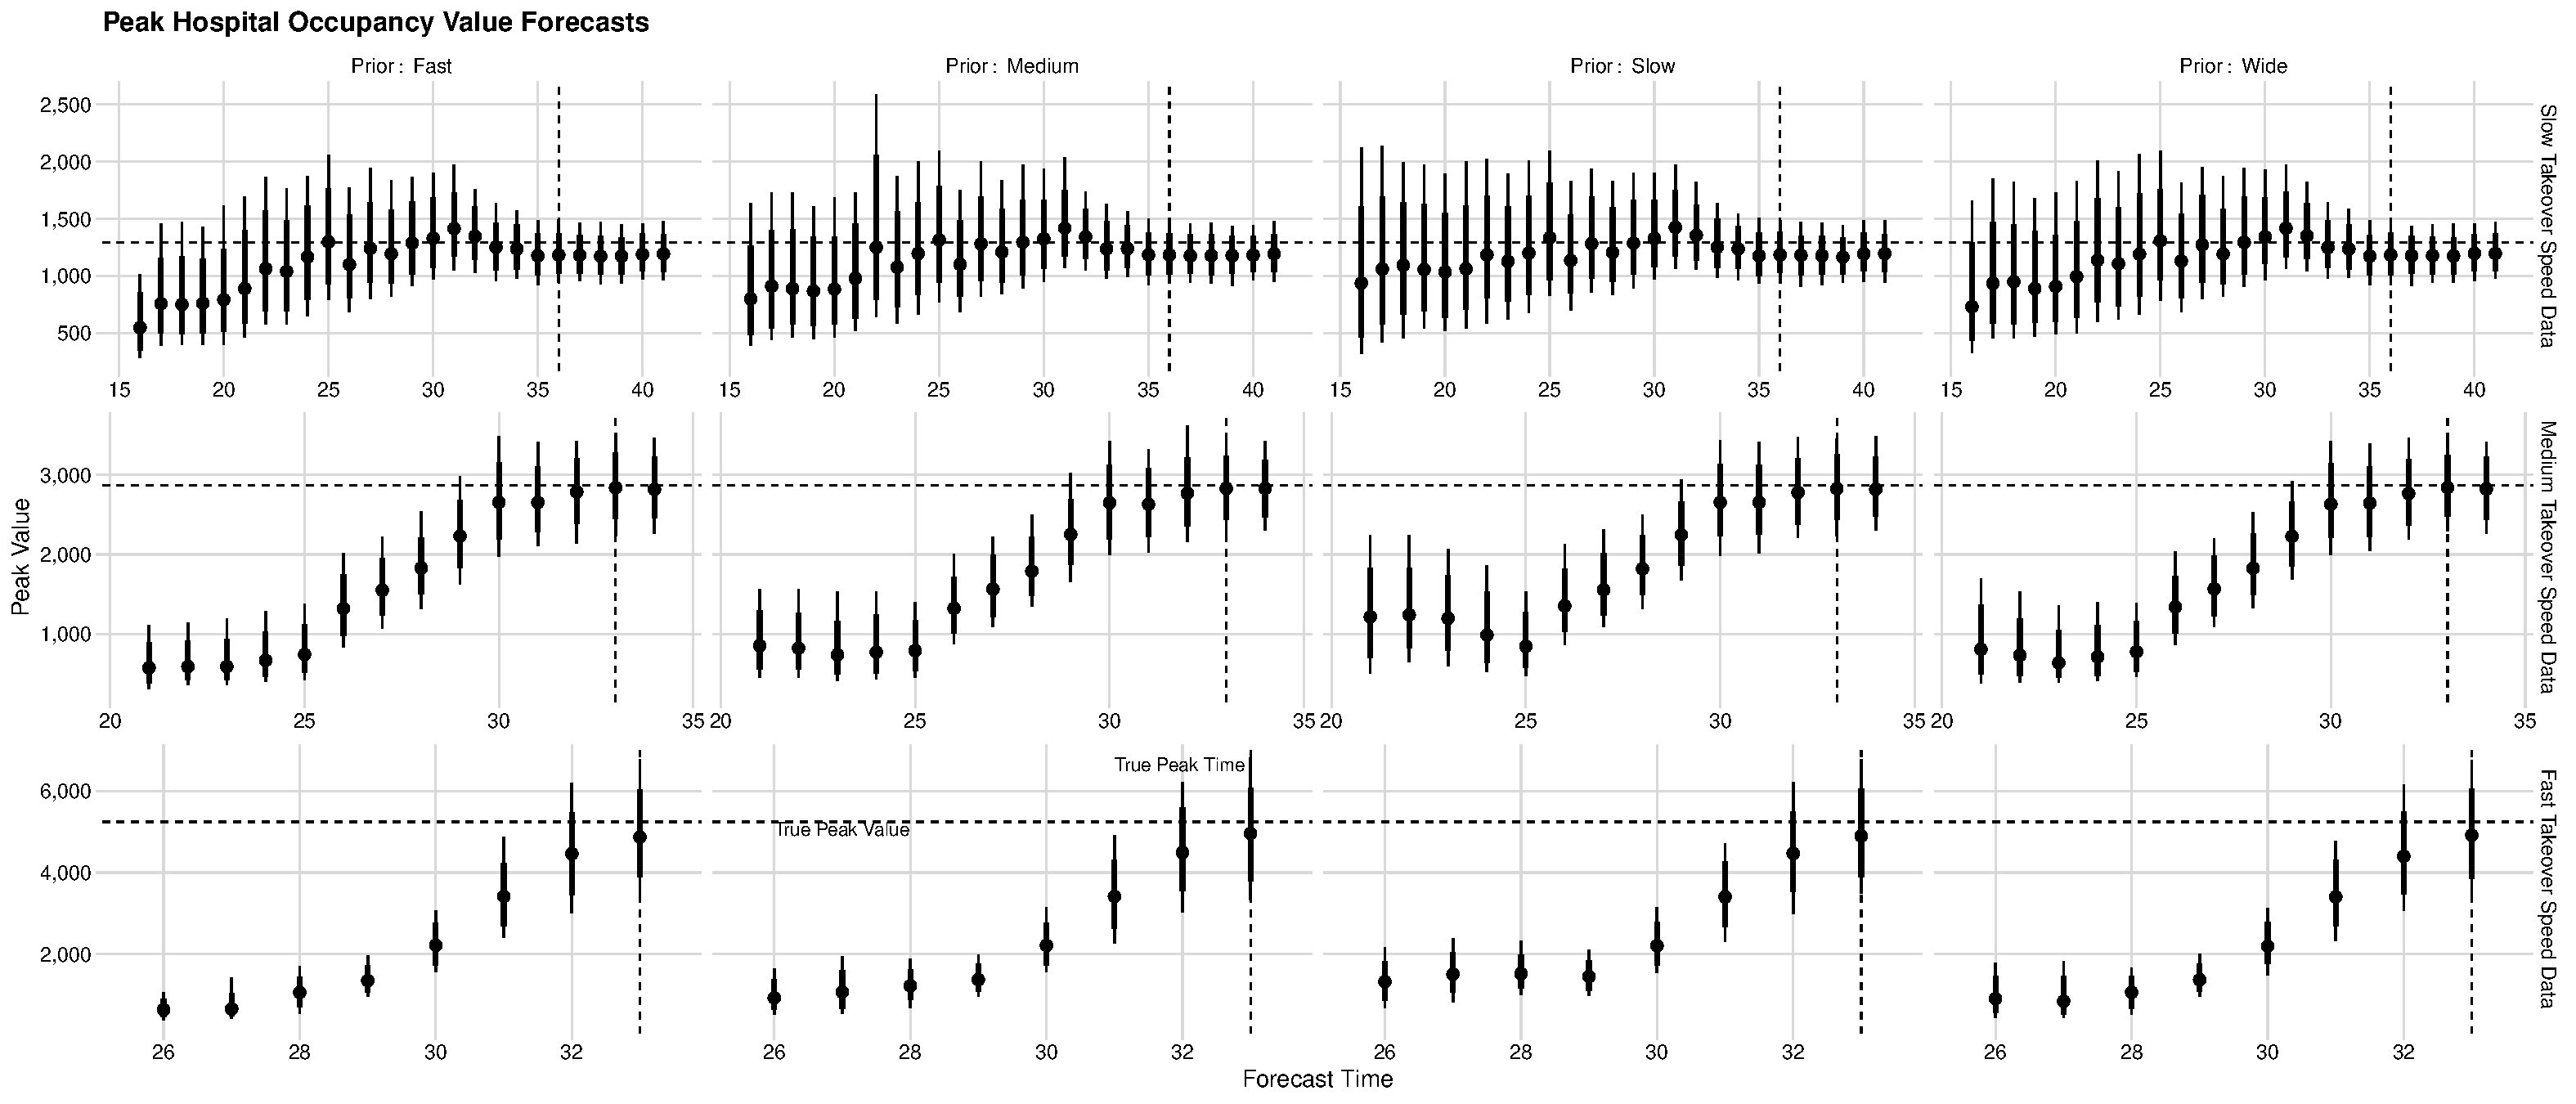
\includegraphics[width=1.0\columnwidth]{sensitivity_simulated_peak_assessment_value_plot}
    \caption[Posterior predictive intervals for peak hospital occupancy for simulated data sets.]{Posterior predictive intervals for the maximum hospital occupancy in three simulated data sets.
    Dots indicate the median of the predictive distribution, while the thick and thin lines represent central 80\% and 95\% intervals, respectively.
    Horizontal dashed lines indicate the true peak hospital occupancy, while the vertical dashed lines indicate the true peak hospital occupancy time.}
    \label{ch_5:fig:sensitivity_simulated_peak_assessment_value_plot}
\end{figure}

\begin{figure}
    \centering
    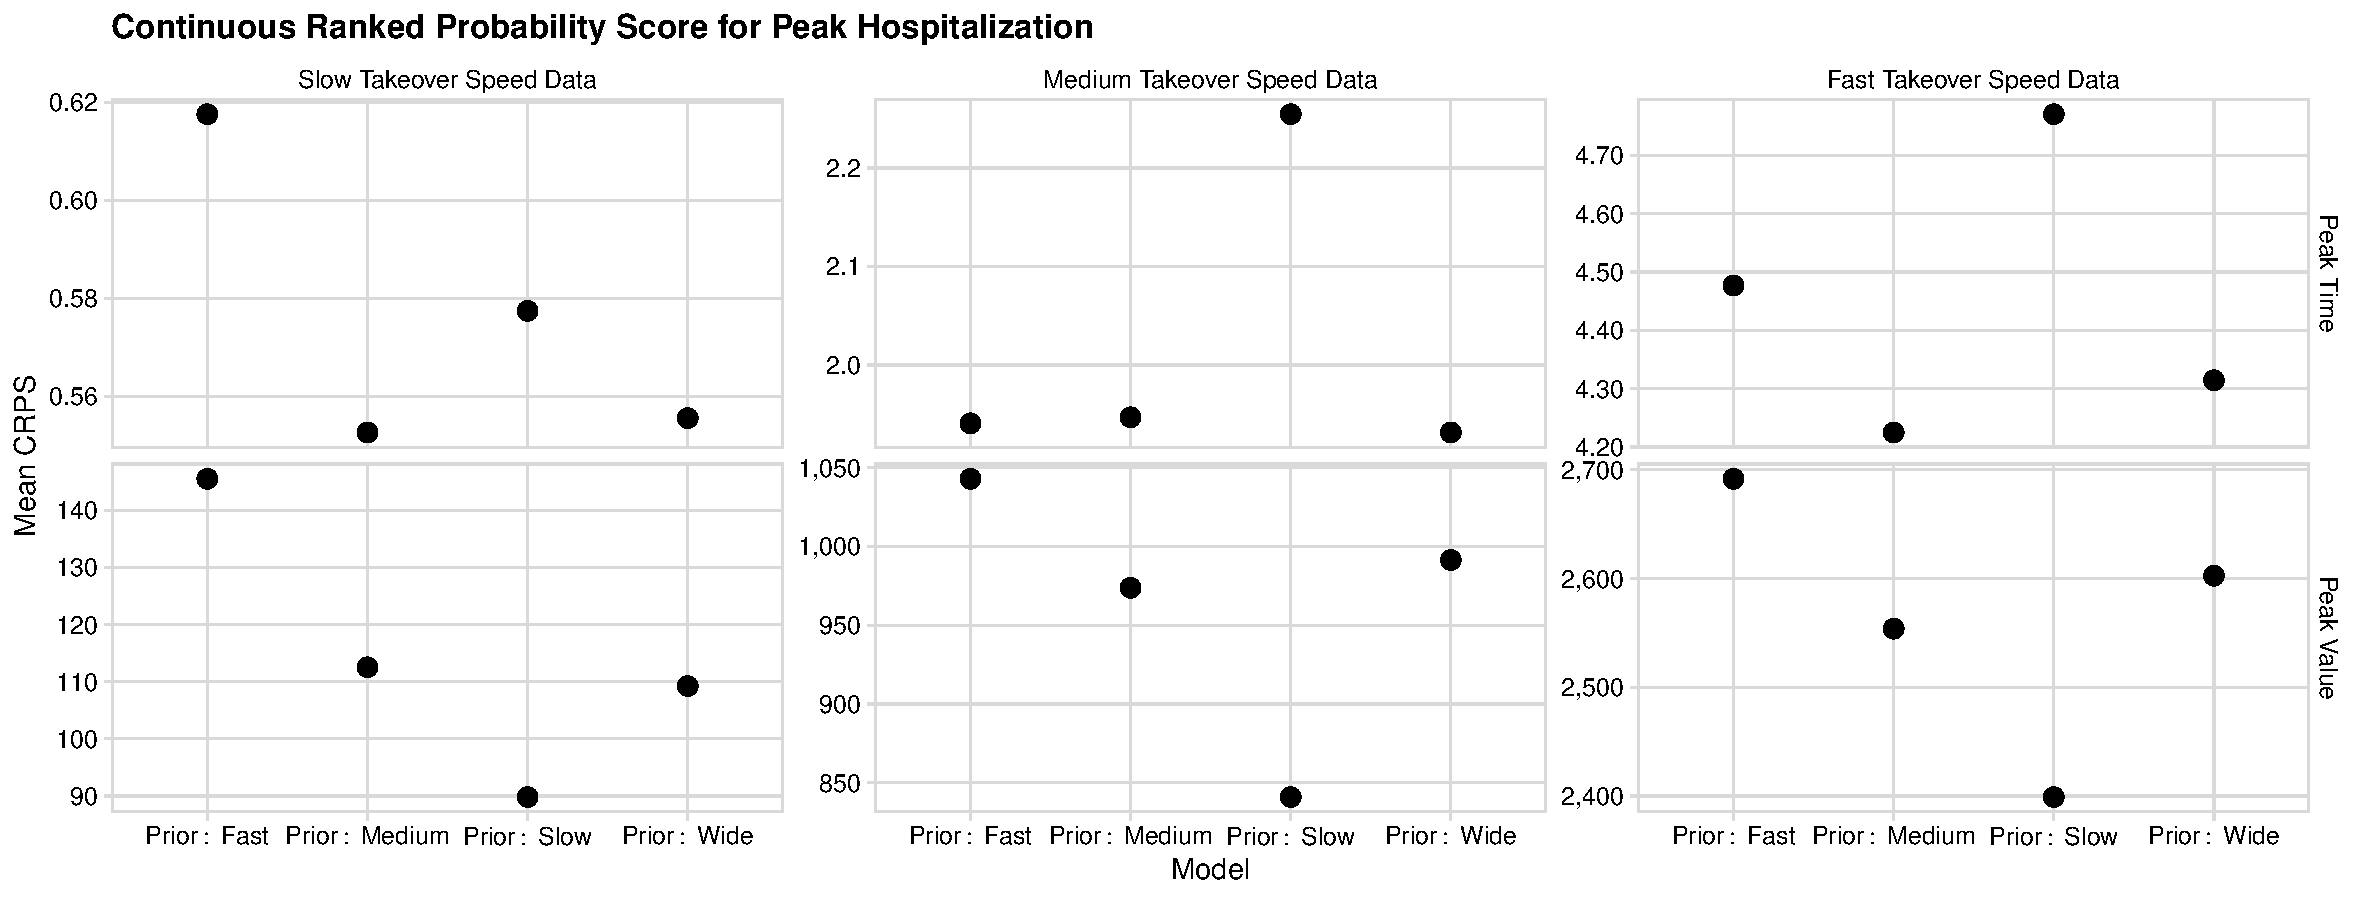
\includegraphics[width=1.0\columnwidth]{sensitivity_simulated_peak_crps_dotplot_plot}
    \caption[CRPS summaries for peak hospital occupancy in simulated data sets.]{CRPS summaries for peak hospital occupancy timing and size for three simulated data sets. Lower CRPS is better.}
    \label{ch_5:fig:sensitivity_simulated_peak_crps_dotplot_plot}
\end{figure}

\section{Additional California data results}

\begin{xltabular}{\columnwidth}{c>{\RaggedRight}Xllc}
    \label{ch_5:tbl:real_data_prior_table}\\
\caption{TKTK}\\[\belowcaptionskip]
	\thead{Parameter} & \thead{Interpretation} & \thead{Prior} & \thead{Prior Median\\ (95\% Interval)} \\ \hline
\end{xltabular}

\begin{figure}
    \centering
    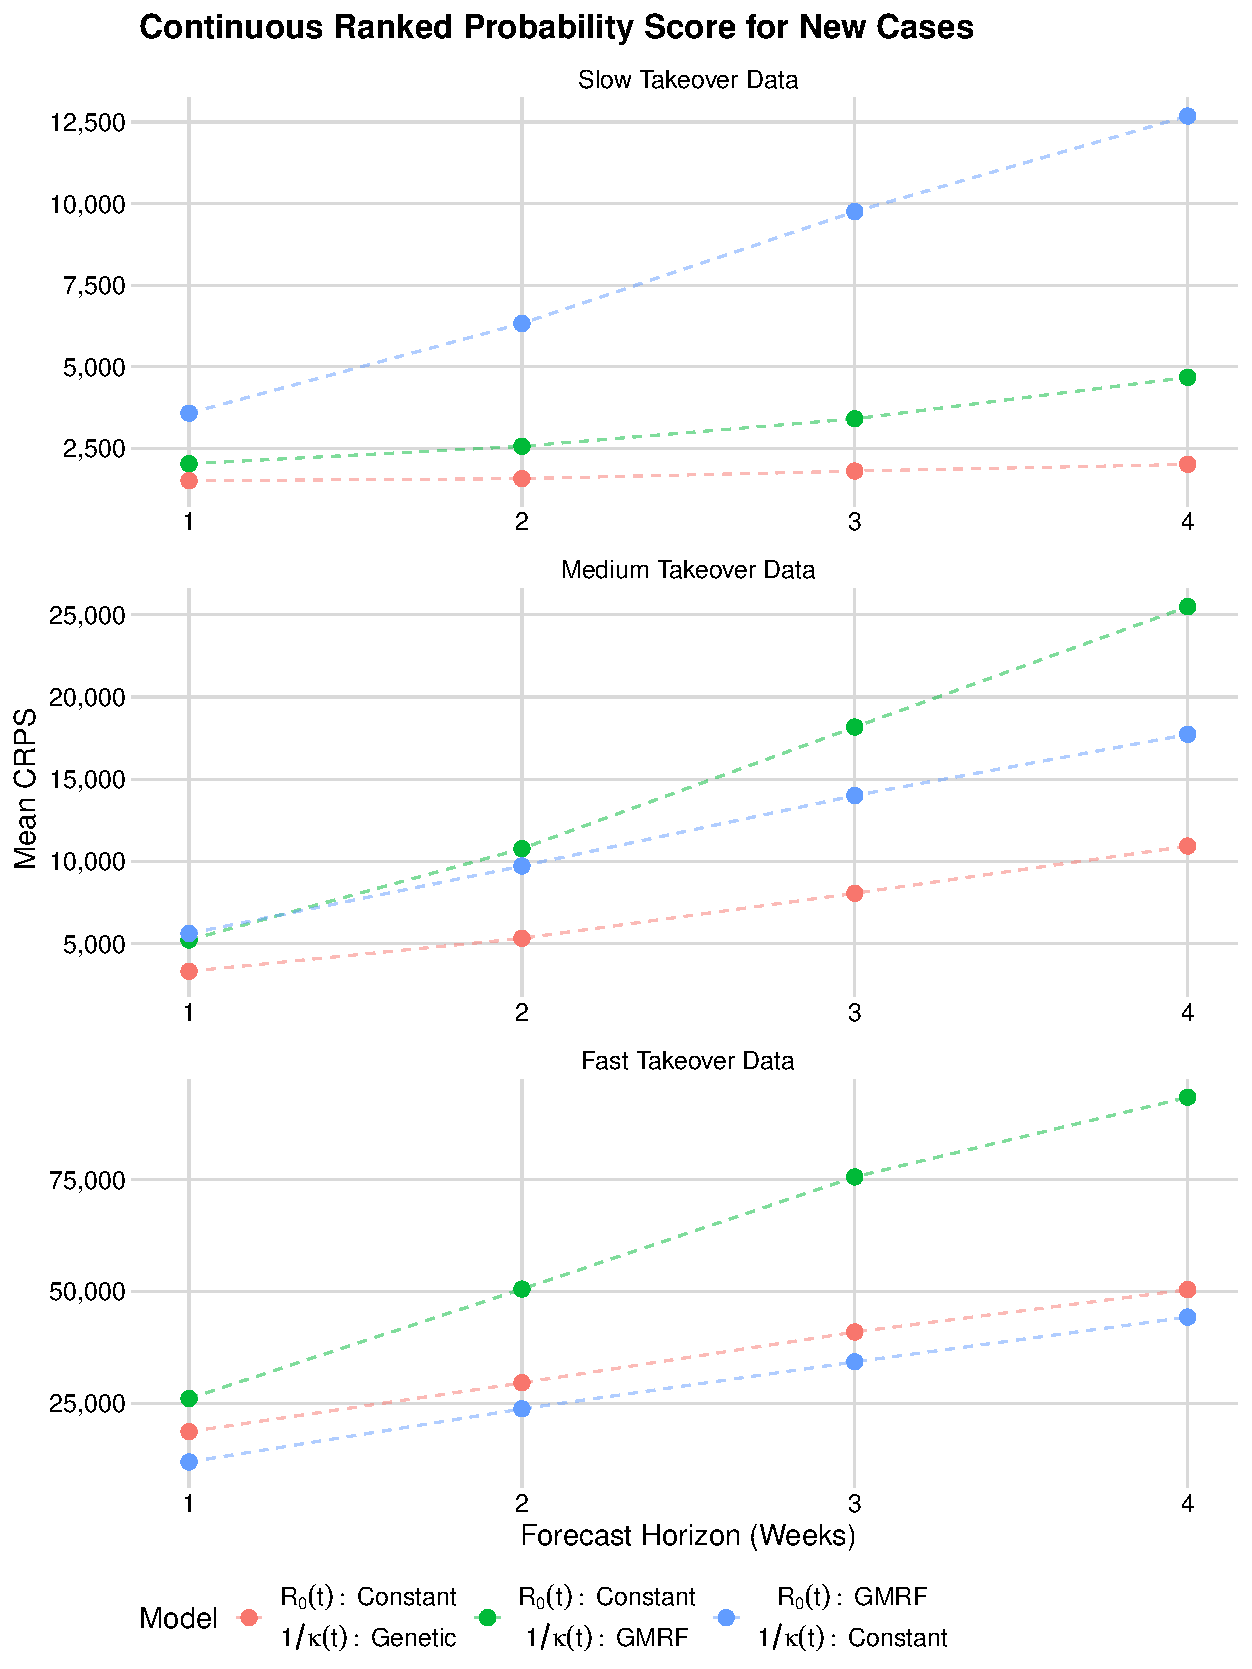
\includegraphics[width=1.0\columnwidth]{real_data_crps_comparison_dotplot_data_new_cases_plot}
    \caption[CRPS summaries for new cases forecasts for real data sets.]{CRPS summaries for new cases forecasts at 1, 2, and 4-week horizons for California and Orange County data sets. Lower CRPS is better.}
    \label{ch_5:fig:real_data_crps_comparison_dotplot_data_new_cases_plot}
\end{figure}

\begin{figure}
    \centering
    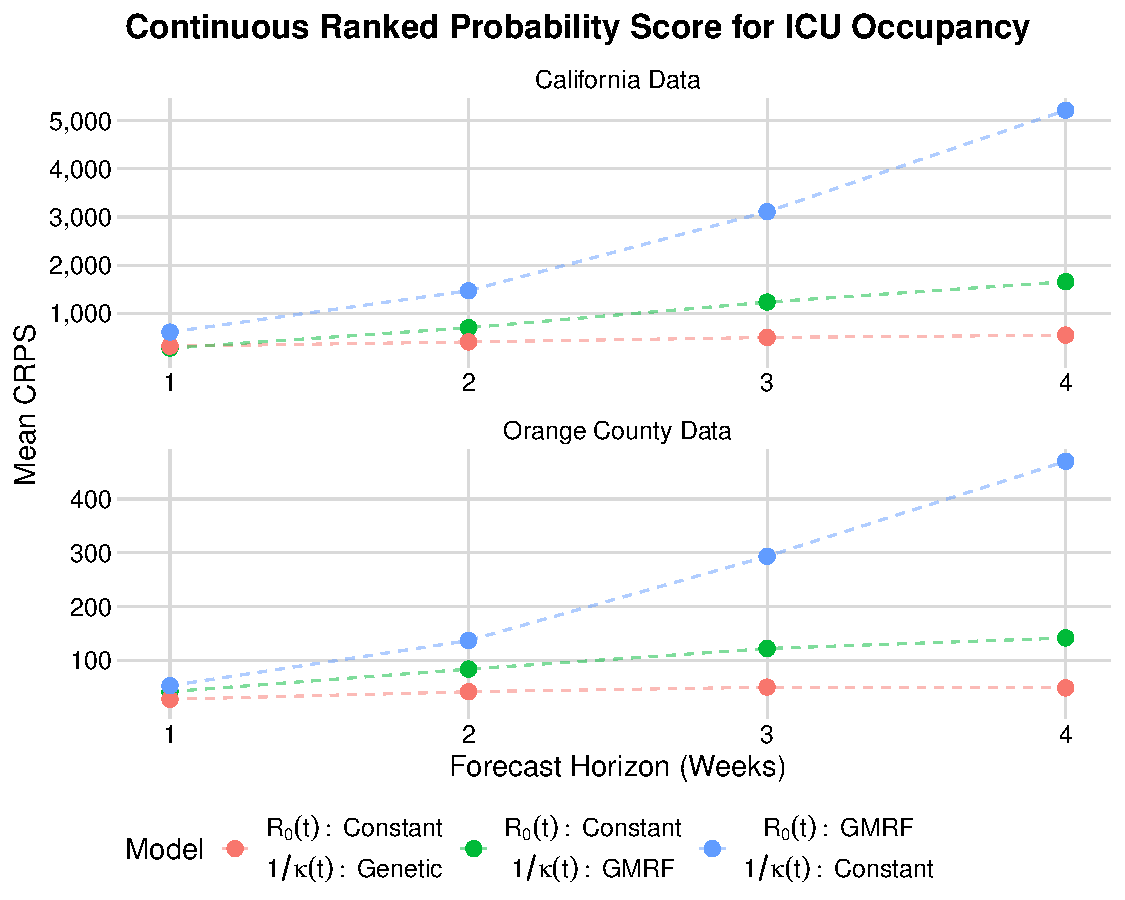
\includegraphics[width=1.0\columnwidth]{real_data_crps_comparison_dotplot_data_icu_plot}
    \caption[CRPS summaries for ICU occupancy forecasts for real data sets.]{CRPS summaries for ICU occupancy forecasts at 1, 2, and 4-week horizons for California and Orange County data sets. Lower CRPS is better.}
    \label{ch_5:fig:real_data_crps_comparison_dotplot_data_icu_plot}
\end{figure}

\begin{figure}
    \centering
    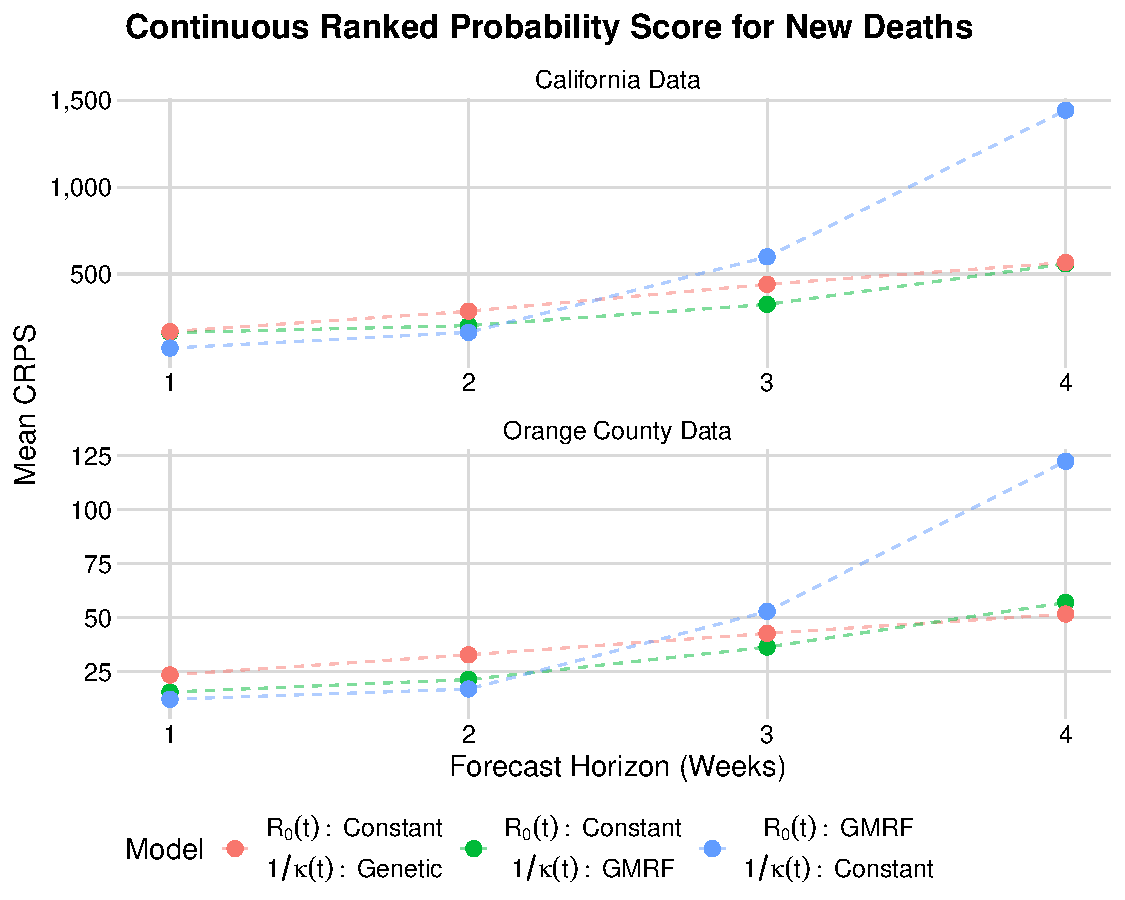
\includegraphics[width=1.0\columnwidth]{real_data_crps_comparison_dotplot_data_new_deaths_plot}
    \caption[CRPS summaries for new deaths occupancy forecasts for real data sets.]{CRPS summaries for new deaths occupancy forecasts at 1, 2, and 4-week horizons for California and Orange County data sets. Lower CRPS is better.}
    \label{ch_5:fig:real_data_crps_comparison_dotplot_data_new_deaths_plot}
\end{figure}

\begin{figure}
    \centering
    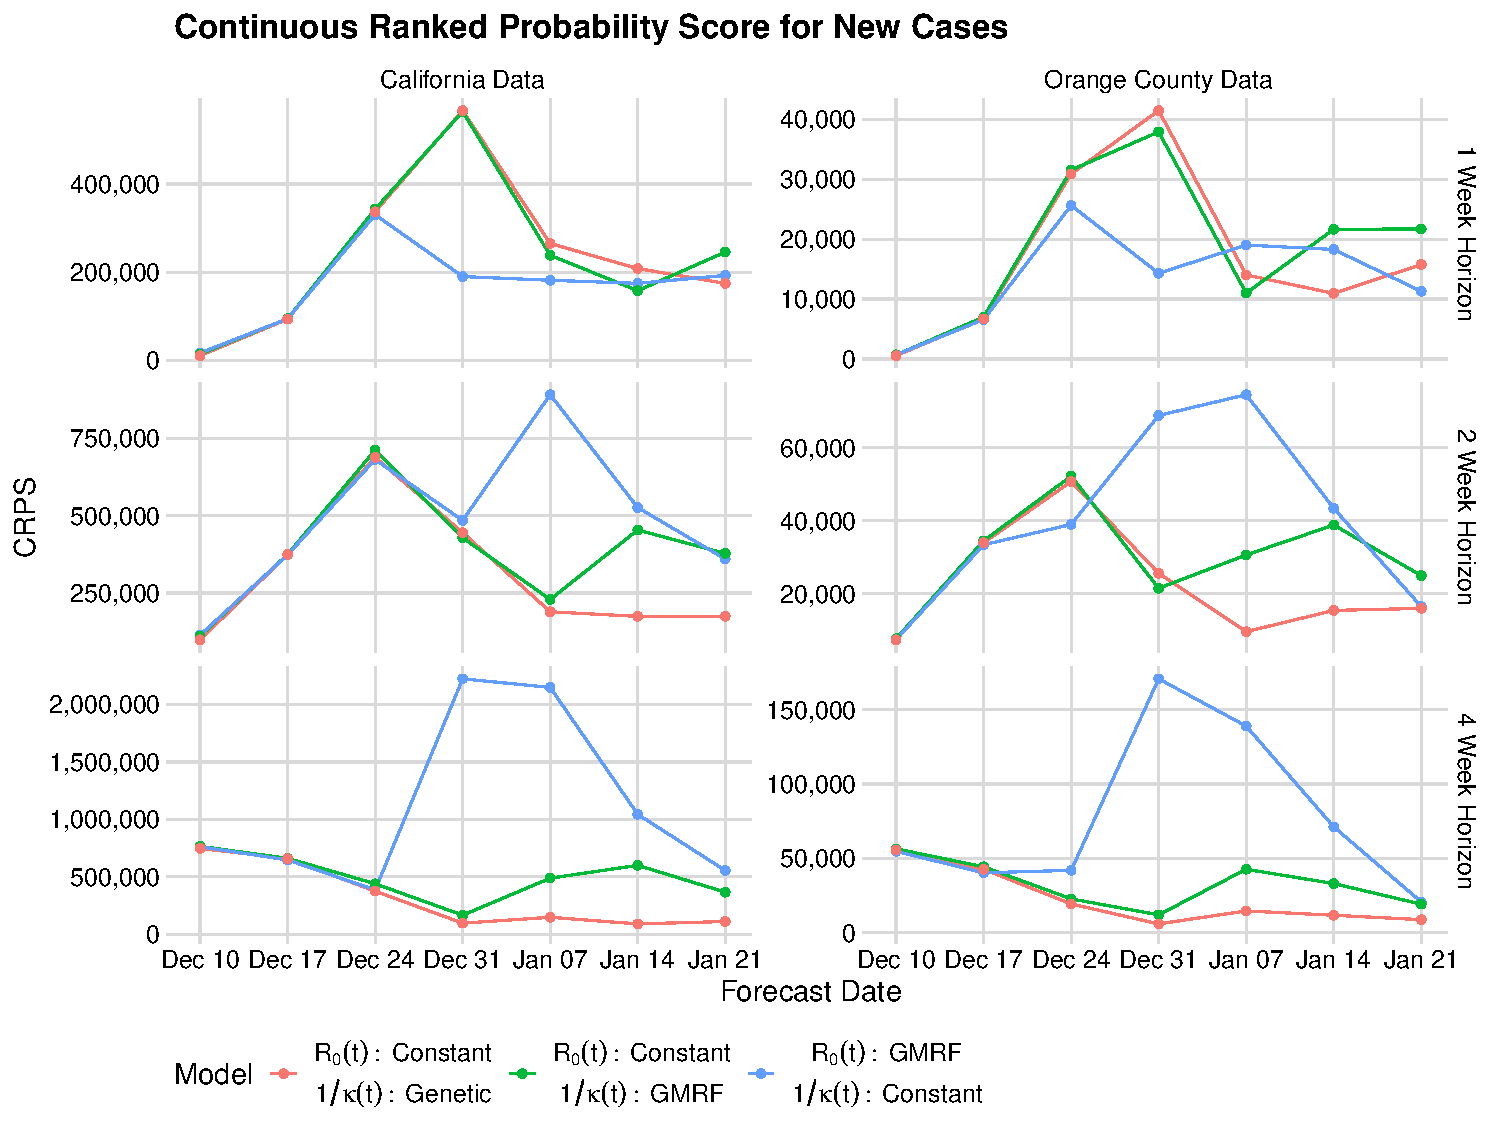
\includegraphics[width=1.0\columnwidth]{real_data_crps_comparison_data_new_cases_plot}
    \caption{Individual CRPS for new cases forecasts at 1, 2, and 4-week horizons for California and Orange County data sets. Lower CRPS is better.}
    \label{ch_5:fig:real_data_crps_comparison_data_new_cases_plot}
\end{figure}

\begin{figure}
    \centering
    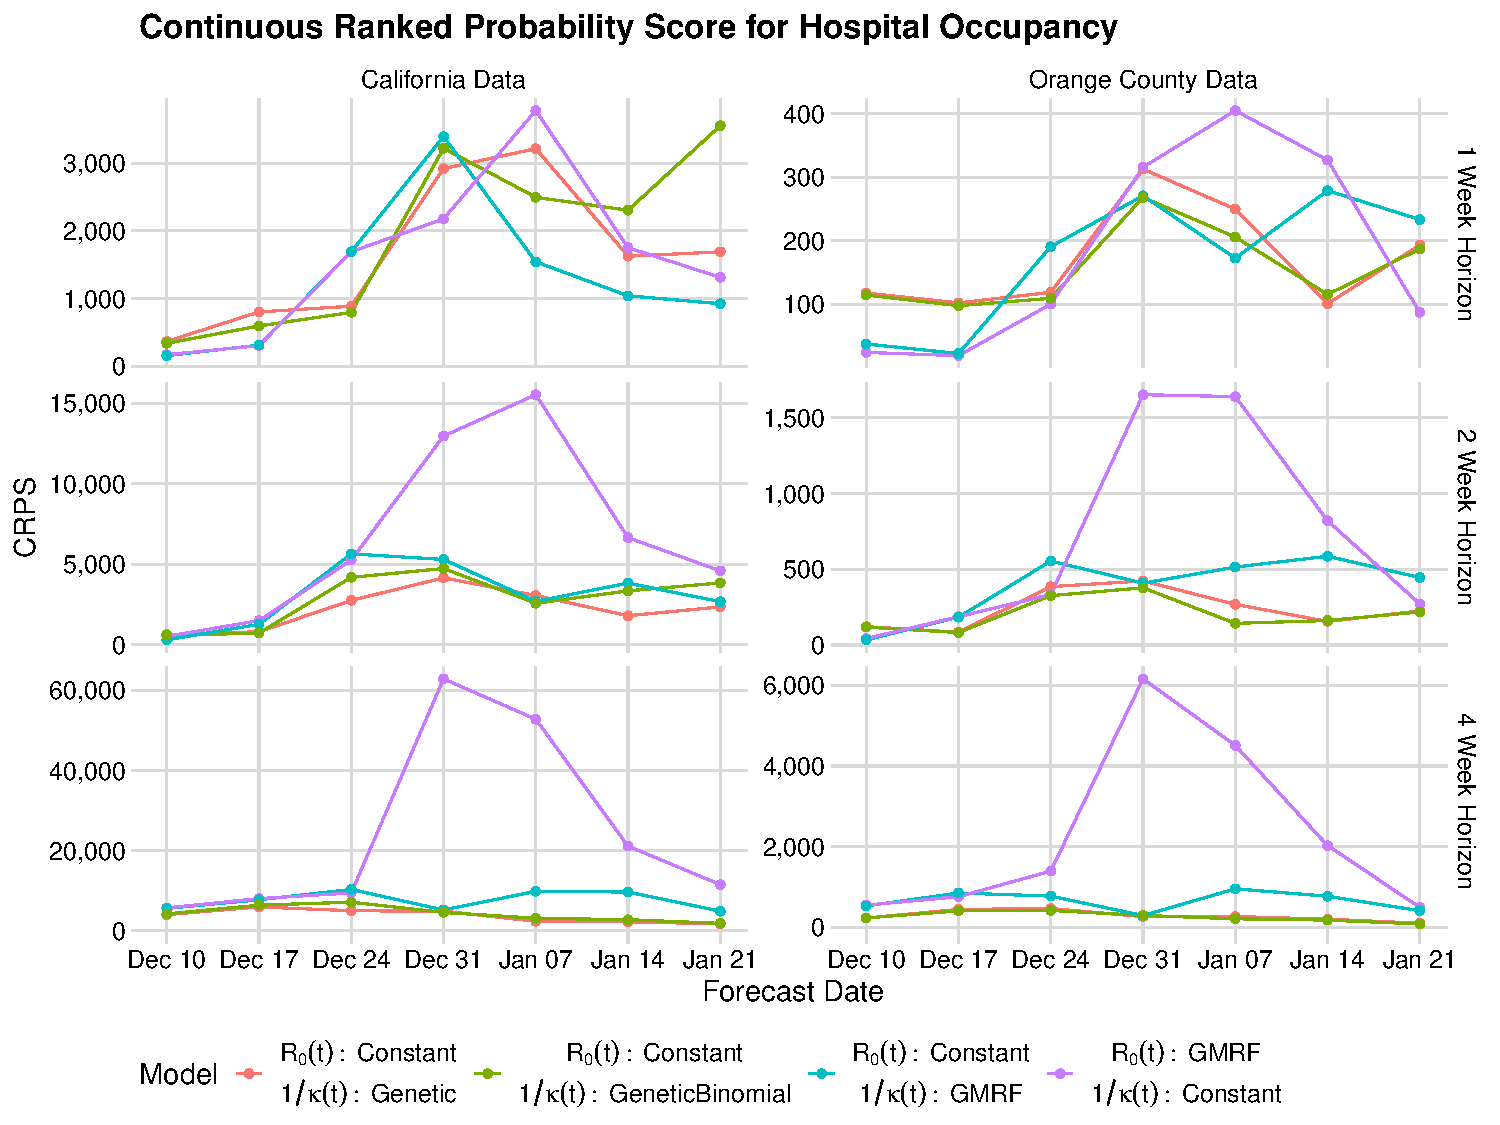
\includegraphics[width=1.0\columnwidth]{real_data_crps_comparison_data_hospitalizations_plot}
    \caption{Individual CRPS for hospital occupancy forecasts at 1, 2, and 4-week horizons for California and Orange County data sets. Lower CRPS is better.}
    \label{ch_5:fig:real_data_crps_comparison_data_hospitalizations_plot}
\end{figure}

\begin{figure}
    \centering
    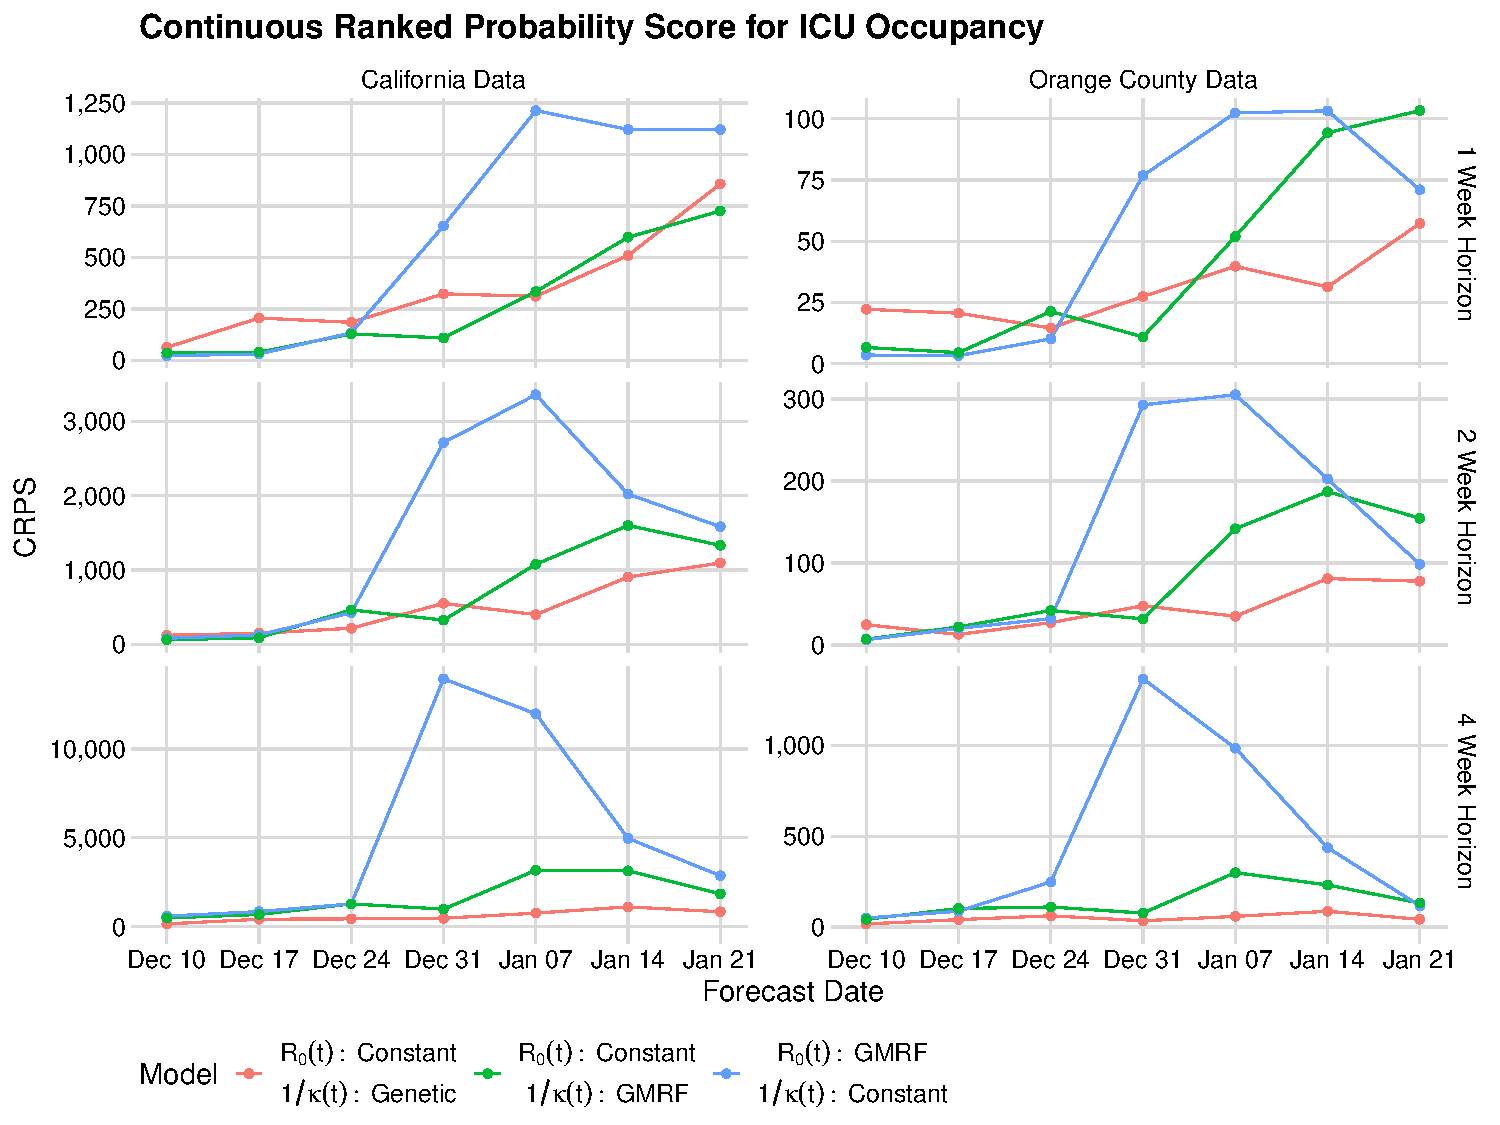
\includegraphics[width=1.0\columnwidth]{real_data_crps_comparison_data_icu_plot}
    \caption{Individual CRPS for ICU occupancy forecasts at 1, 2, and 4-week horizons for California and Orange County data sets. Lower CRPS is better.}
    \label{ch_5:fig:real_data_crps_comparison_data_icu_plot}
\end{figure}

\begin{figure}
    \centering
    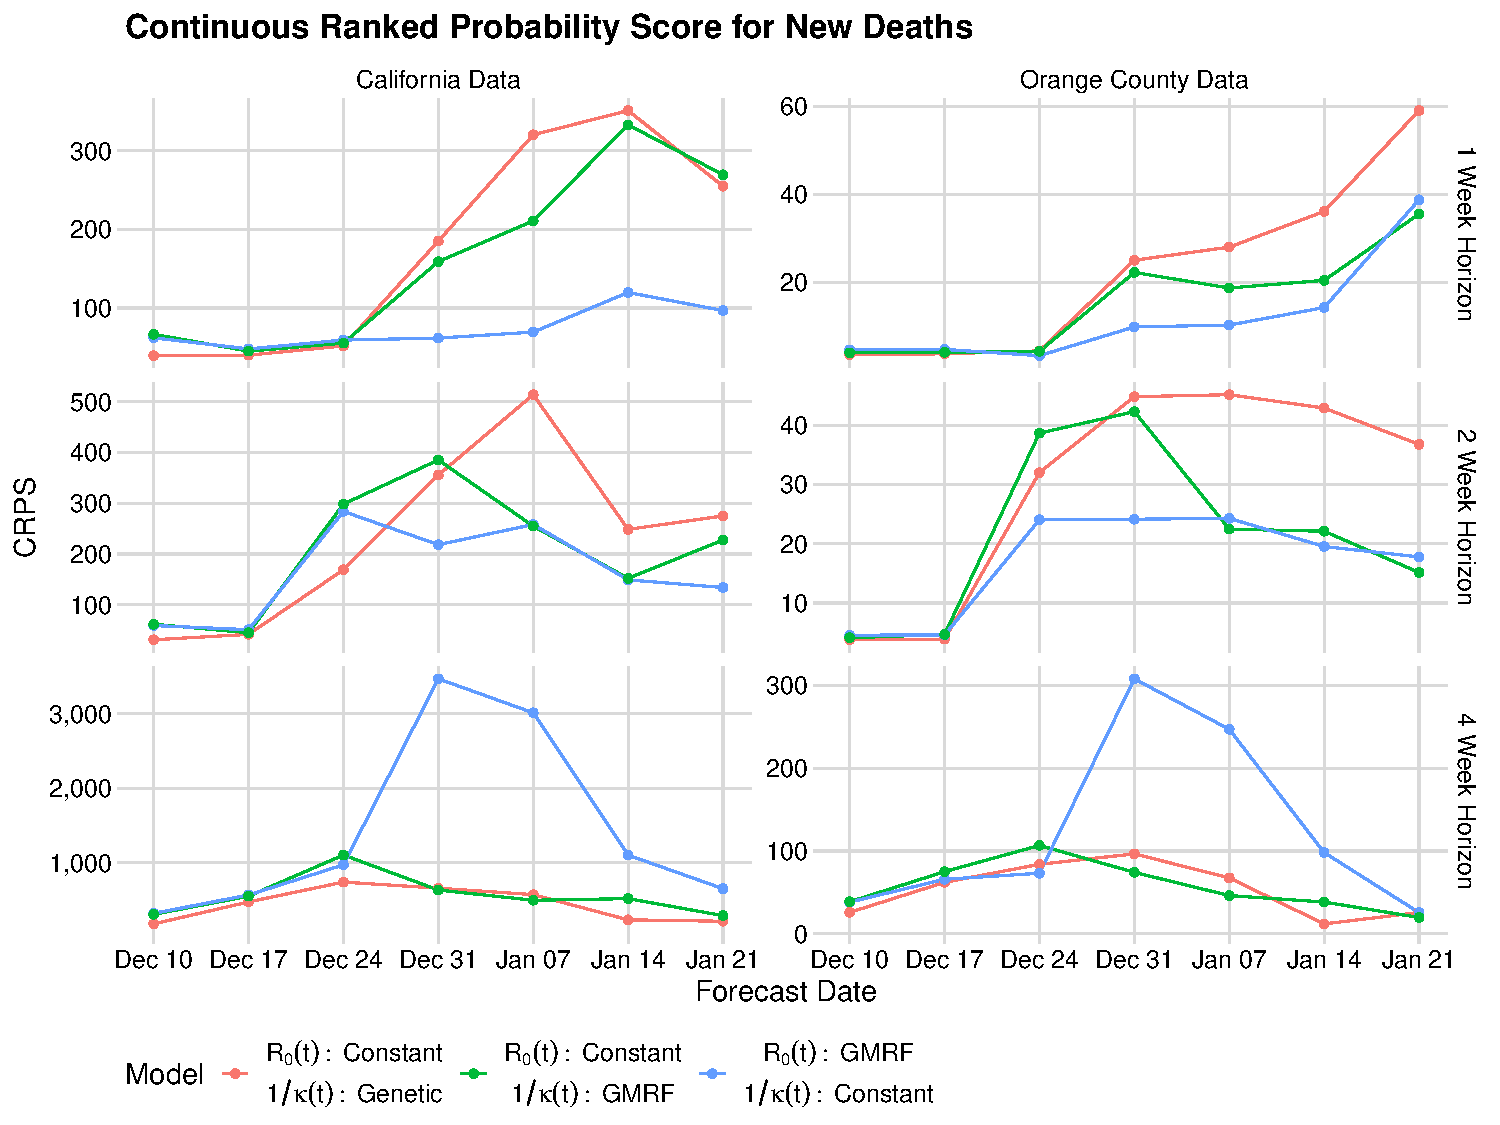
\includegraphics[width=1.0\columnwidth]{real_data_crps_comparison_data_new_deaths_plot}
    \caption{Individual CRPS for new deaths forecasts at 1, 2, and 4-week horizons for California and Orange County data sets. Lower CRPS is better.}
    \label{ch_5:fig:real_data_crps_comparison_data_new_deaths_plot}
\end{figure}

\begin{figure}
    \centering
    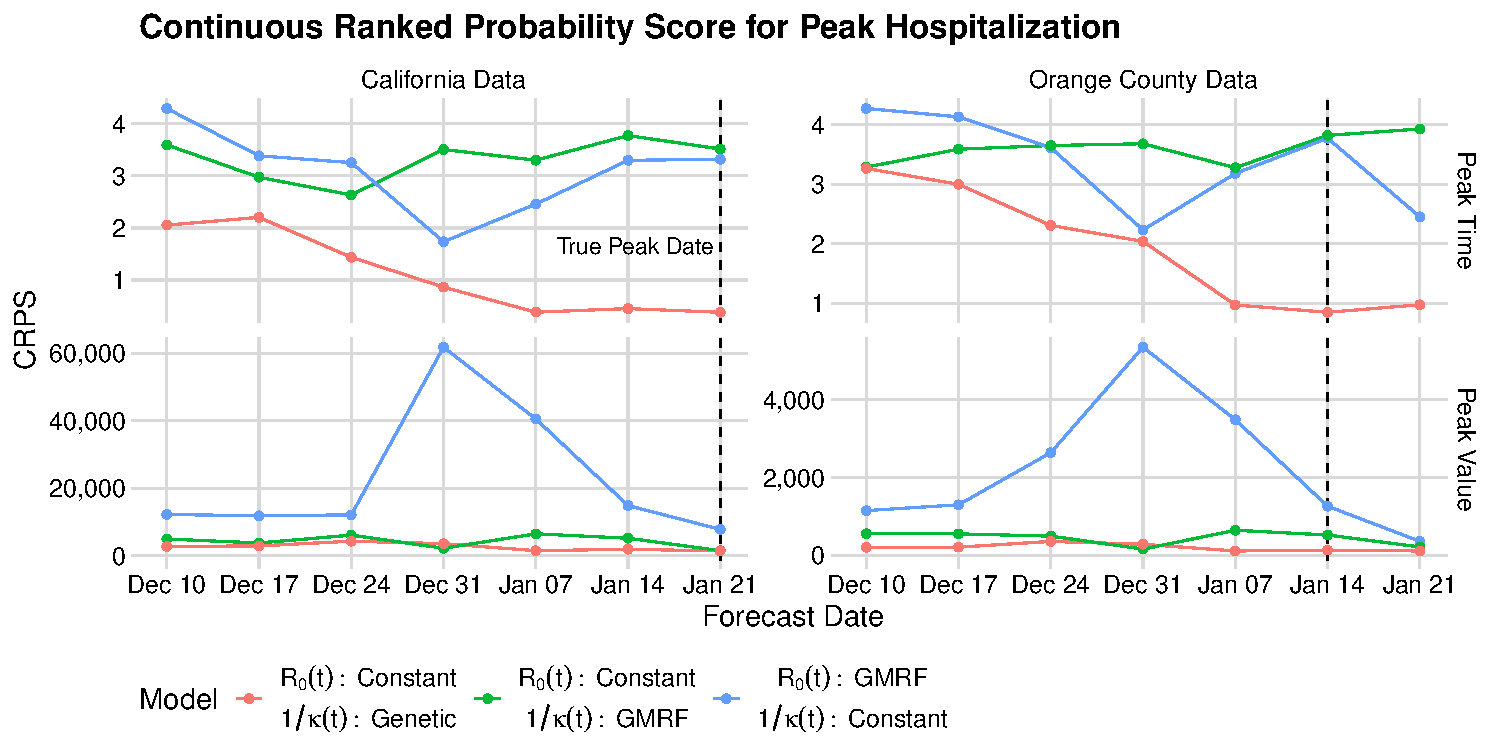
\includegraphics[width=1.0\columnwidth]{real_data_peak_crps_plot}
    \caption[Individual CRPS for peak hospital occupancy in real data sets.]{Individual CRPS for peak hospital occupancy timing and size in California and Orange County data sets. Lower CRPS is better.}
    \label{ch_5:fig:real_data_peak_crps_plot}
\end{figure}

\label{ch_5:sec:real_cases_icu_death}

\addtocontents{toc}{\protect\setcounter{tocdepth}{2}}